%% abtex2-modelo-trabalho-academico.tex, v-1.7.1 laurocesar
%% Copyright 2012-2013 by abnTeX2 group at http://abntex2.googlecode.com/ 
%%
%% This work may be distributed and/or modified under the
%% conditions of the LaTeX Project Public License, either version 1.3
%% of this license or (at your option) any later version.
%% The latest version of this license is in
%%   http://www.latex-project.org/lppl.txt
%% and version 1.3 or later is part of all distributions of LaTeX
%% version 2005/12/01 or later.
%%
%% This work has the LPPL maintenance status `maintained'.
%% 
%% The Current Maintainer of this work is the abnTeX2 team, led
%% by Lauro César Araujo. Further information are available on 
%% http://abntex2.googlecode.com/
%%
%% This work consists of the files abntex2-modelo-trabalho-academico.tex,
%% abntex2-modelo-include-comandos and abntex2-modelo-references.bib
%%

% ------------------------------------------------------------------------
% ------------------------------------------------------------------------
% abnTeX2: Modelo de Trabalho Academico (tese de doutorado, dissertacao de
% mestrado e trabalhos monograficos em geral) em conformidade com 
% ABNT NBR 14724:2011: Informacao e documentacao - Trabalhos academicos -
% Apresentacao
% ------------------------------------------------------------------------
% ------------------------------------------------------------------------
%
% ------------------------------------------------------------------------
% ------------------------------------------------------------------------
% ufsj-abnTeX2: Modelo de Trabalho Academico do Departamento de Ciência
% da Computação da UFSJ
% Derivado da classe ABNTex, em conformidade com ABNT NBR 14724:2011
% Informacao e documentacao - Trabalhos academicos - Apresentacao
% ------------------------------------------------------------------------
% ------------------------------------------------------------------------

% TODO: Comentários da primeira apresentação
% - Fazer quadro comparativo com trabalhos mais semelhantes da literatura;
%   Colunas para o quadro: Representação gráfica do modelo | Distribuição do Software (web, desktop) | Tipos de modelos simulados | Acesso ao código usado na simulação | Simulação interativa
%      VCell, InsightMaker, Snoopy, BioDynaMo
% - Destacar o ensino-aprendizagem: introdução
% - explicar o template (ex: o Jinja possuí estruturas de controles, laços, breve explicação do código sendo executado)
% - imagens do software na metodologia
% - sec "Geração de Código e Simulação interativa": 

% Fix taken from: https://build.opensuse.org/request/show/973887
% Apparently, hyperref doesn't ship with htmladdnormallink anymore
\ifdefined\htmladdnormallink\relax\else%
\def\htmladdnormallink#1#2{\href{#2}{#1}}
\fi

\documentclass[
	% -- opções da classe memoir --
	12pt,				% tamanho da fonte
	openright,			% capítulos começam em pág ímpar (insere página vazia caso preciso)
	oneside,			% para impressão em verso e anverso. Oposto a oneside
	a4paper,			% tamanho do papel. 
	% -- opções da classe abntex2 --
	%chapter=TITLE,		% títulos de capítulos convertidos em letras maiúsculas
	%section=TITLE,		% títulos de seções convertidos em letras maiúsculas
	%subsection=TITLE,	% títulos de subseções convertidos em letras maiúsculas
	%subsubsection=TITLE,% títulos de subsubseções convertidos em letras maiúsculas
	% -- opções do pacote babel --
	main=brazil,
	english,			% idioma adicional para hifenização
	%french,				% idioma adicional para hifenização
	%spanish,			% idioma adicional para hifenização
	%brazil,				% o último idioma é o principal do documento
	]{ufsj-abntex2}


% ---
% PACOTES
% ---
\usepackage{amsmath}
\usepackage{subfig}
\usepackage{listings}
\usepackage{listingsutf8}
\usepackage{xcolor}
\usepackage{colortbl}
\usepackage{nicefrac, xfrac}
\usepackage{attachfile2}
\definecolor{codegreen}{rgb}{0,0.6,0}
\definecolor{codegray}{rgb}{0.5,0.5,0.5}
\definecolor{codepurple}{rgb}{0.58,0,0.82}
\definecolor{backcolour}{rgb}{1, 1, 1}    %{0.95,0.95,0.92}

\lstdefinestyle{mystyle}{
    backgroundcolor=\color{backcolour},   
    commentstyle=\color{codegreen},
    keywordstyle=\color{magenta},
    numberstyle=\tiny\color{codegray},
    stringstyle=\color{codepurple},
    basicstyle=\ttfamily\footnotesize,
    breakatwhitespace=false,         
    breaklines=true,                 
    captionpos=b,                    
    keepspaces=true,                 
    numbers=left,                    
    numbersep=5pt,                  
    showspaces=false,                
    showstringspaces=false,
    showtabs=false,                  
    tabsize=2
}
\lstset{
    style=mystyle, 
    inputencoding=utf8
}
% ---
% Pacotes fundamentais 
% ---
\usepackage{cmap}				% Mapear caracteres especiais no PDF
\usepackage{lmodern}			% Usa a fonte Latin Modern			
\usepackage[T1]{fontenc}		% Selecao de codigos de fonte.
\usepackage[utf8]{inputenc}		% Codificacao do documento (conversão automática dos acentos)
\usepackage{comment}

\usepackage{lastpage}			% Usado pela Ficha catalográfica
\usepackage{indentfirst}		% Indenta o primeiro parágrafo de cada seção.
\usepackage{color}				% Controle das cores
\usepackage{graphicx}			% Inclusão de gráficos
\usepackage{float}
\usepackage[alf]{abntex2cite}	% Citações padrão ABNT

% ---
	

\begin{comment}
% ---
% Pacotes de citações
% ---
\usepackage[brazilian,hyperpageref]{backref}	 % Paginas com as citações na bibl


% --- 
% CONFIGURAÇÕES DE PACOTES
% --- 

% ---
% Configurações do pacote backref
% Usado sem a opção hyperpageref de backref
\renewcommand{\backrefpagesname}{Citado na(s) página(s):~}
% Texto padrão antes do número das páginas
\renewcommand{\backref}{}
% Define os textos da citação
\renewcommand*{\backrefalt}[4]{
	\ifcase #1 %
		Nenhuma citação no texto.%
	\or
		Citado na página #2.%
	\else
		Citado #1 vezes nas páginas #2.%
	\fi}%
% ---
\end{comment}

%se desejar que nas referências a página que o trabalho foi citado, descomentar aqui acima da linha 80 ate a 108


% ---------------------------------------------------------------------------------------------
% ---------------------------------------------Informações de dados para CAPA e FOLHA DE ROSTO-
% ---------------------------------------------------------------------------------------------
\titulo{Desenvolvimento de um software científico para a modelagem e simulação computacional}
\autor{Brenno Lemos Melquiades}
\local{São João del-Rei}
\data{\the\year}
\orientador{Alexandre Bittencourt Pigozzo}
%\coorientador{Nome do Co-orientador} % se não existir, comente essa linha
\instituicao{%
  Universidade Federal de São João del-Rei — UFSJ
  \par
  Pós-Graduação em Ciência da Computação}
\tipotrabalho{Dissertação de Mestrado}
% O preambulo deve conter o tipo do trabalho, o objetivo, 
% o nome da instituição e a área de concentração 
\preambulo{Qualificação apresentada como requisito para obtenção do título de Mestre em Ciência da Computação do curso de mestrado do Programa de Pós Graduação em Ciência da Computação (PPGCC) da UFSJ.}
% ---


% ---
% Configurações de aparência do PDF final

% alterando o aspecto da cor azul
\definecolor{blue}{RGB}{41,5,195}

% informações do PDF
\makeatletter
\hypersetup{
     	%pagebackref=true,
		pdftitle={\@title}, 
		pdfauthor={\@author},
    	pdfsubject={\imprimirpreambulo},
	    pdfcreator={LaTeX with abnTeX2},
		pdfkeywords={UFSJ}{DCOMP}{ufsj-abntex2}{trabalho acadêmico}, 
		colorlinks=true,       		% false: boxed links; true: colored links
    	linkcolor=blue,          	% color of internal links
    	citecolor=blue,        		% color of links to bibliography
    	filecolor=magenta,      		% color of file links
		urlcolor=blue,
		bookmarksdepth=4
}
\makeatother
% --- 

% --- 
% Espaçamentos entre linhas e parágrafos 
% --- 
% O tamanho do parágrafo é dado por:
\setlength{\parindent}{1.3cm}
% Controle do espaçamento entre um parágrafo e outro:
\setlength{\parskip}{0.2cm}  % tente também \onelineskip

% ---
% compila o indice
% ---
\makeindex

% -----------------------------------------------------------------------------------
% -----------------------------------------------------------------------------------
% -----------------------------------------------------------------------------------
% ---------------------------------------------------------------Início do documento-
% -----------------------------------------------------------------------------------
% -----------------------------------------------------------------------------------
% -----------------------------------------------------------------------------------
\begin{document}

% Retira espaço extra obsoleto entre as frases.
\frenchspacing 

% -----------------------------------------------------------------------------------
% ------------------------------------------------------------ELEMENTOS PRÉ-TEXTUAIS-
% -------------------------------------------Altere o arquivo 00_pretextual.tex para-
% ---------------folha de aprovação, dedicatória, agradecimento e epígrafe e resumos-
% -----------------------------------------------------------------------------------
\pretextual

% ---------------------------------------------------------------------------------------------
% ----------------------------------------------------------------------------------------Capa-
% ---------------------------------------------------------------------------------------------
\imprimircapa
% ---

% ---------------------------------------------------------------------------------------------
% ------------------------------------------------------------------------------Folha de rosto-
% ---------------------------------------------------------------------------------------------
\imprimirfolhaderosto

% ---------------------------------------------------------------------------------------------
% --------------------------------------------------------------------------Folha de aprovação-
% -------------------------------------------------------Dedicatória, Agradecimento e Epígrafe-
% --------------------------------------------------------------Resumos, em português e inglês-
% ---------------------------------------------------------------------------------------------
% Isto é um exemplo de Folha de aprovação, elemento obrigatório da NBR
% 14724/2011 (seção 4.2.1.3). Você pode utilizar este modelo até a aprovação
% do trabalho. Após isso, substitua todo o conteúdo deste arquivo por uma
% imagem da página assinada pela banca com o comando abaixo:
%
% \includepdf{folhadeaprovacao_final.pdf}
%
\begin{folhadeaprovacao}

  \begin{center}
    {\ABNTEXchapterfont\large\imprimirautor}

    \vspace*{\fill}\vspace*{\fill}
    {\ABNTEXchapterfont\bfseries\Large\imprimirtitulo}
    \vspace*{\fill}
    
    \hspace{.45\textwidth}
    \begin{minipage}{.5\textwidth}
        \imprimirpreambulo
    \end{minipage}%
    \vspace*{\fill}
   \end{center}
    
   \imprimirlocal, \today
   % Caso prefira fixar a data, basta mudar o comando \today pela data,
   %   como no exemplo abaixo:
   %Trabalho aprovado. \imprimirlocal, 7 de setembro de 1822:

   \assinatura{\textbf{\imprimirorientador} \\ Orientador} 
   \assinatura{\textbf{Prof. Rafael Sachetto Oliveira} \\ Convidado 1}
   \assinatura{\textbf{Prof. Marcelo Lobosco} \\ Convidado 2} 
   \assinatura{\textbf{Profa. Bárbara de Melo Quintela} \\ Convidado 3}   
      
   \begin{center}
    \vspace*{0.5cm}
    {\large\imprimirlocal}
    \par
    {\large\imprimirdata}
    \vspace*{1cm}
  \end{center}
  
\end{folhadeaprovacao}

% % ---------------------------------------------------------------------------------------------
% % ---------------------------------------------------------------------------------Dedicatória-
% % ---------------------------------------------------------------------------------------------
% \begin{dedicatoria}
% 	\vspace*{\fill}
% 	\centering
% 	\noindent
% 	\textit{ Este trabalho é dedicado às crianças adultas que,\\
% 		quando pequenas, sonharam em se tornar cientistas.} \vspace*{\fill}
% \end{dedicatoria}

% ---------------------------------------------------------------------------------------------
% ------------------------------------------------------------------------------Agradecimentos-
% ---------------------------------------------------------------------------------------------
\begin{agradecimentos}
Gostaria de agradecer e dedicar este trabalho:

\noindent
Aos meus pais, pelas oportunidades que me deram, pelo apoio nas escolhas que fiz para chegar aqui, pelo companheirismo e pelo amor incondicional que me proporcionaram.

\noindent
Ao meu orientador, Alexandre Pigozzo, que me introduziu ao meio científico, ao tema deste trabalho e me auxiliou não somente neste trabalho, como contribuidor e orientador, mas na minha trajetória nesta universidade.

\noindent
Aos servidores do DCOMP-UFSJ, que mantém um alto nível de educação e demonstram respeito e empatia pelos docentes do curso. Em especial, um agradecimento aos servidores(as) Carolina Xavier, Leonardo Rocha, Marcos Laia, Michelli Loureiro e Douglas Dinalli.

\noindent
Aos meus amigos de Guarapari, que sempre estiveram ao meu lado.

\noindent
À minha namorada, Keina Takashiba, minha melhor amiga, que me ajuda a me organizar e me apoia em tudo que for.

\noindent
Aos amigos que fiz aqui, na UFSJ, Arthur Gabriel Matos, Ana Clara Medina, Lucas Grandolpho e Wesley Guimarães, meus grandes companheiros de trabalhos.

\noindent
À FAPEMIG, que apoiou este e os projetos anteriores.

\noindent
Aos meus colegas e contribuidores do projeto, Diego Augusto Silva Castro, Sávio Francisco Cirino da Paz e Davi Jannotti Coelho Pinheiro.

\noindent
À todos aqueles que apoiam, defendem e lutam por uma educação gratuita e de qualidade para todos.
	
\end{agradecimentos}

% ---------------------------------------------------------------------------------------------
% ------------------------------------------------------------------------------------Epígrafe-
% ---------------------------------------------------------------------------------------------
\begin{epigrafe}
	\vspace*{\fill}
	\begin{flushright}

		
	\end{flushright}
\end{epigrafe}
% ---

% ---------------------------------------------------------------------------------------------
% -------------------------------------------------------------------------resumo em português-
% ---------------------------------------------------------------------------------------------
\begin{resumo}
	
	% TODO: Está exatamente igual ao trabalho de AC, com exceção da nomenclatura. Devemos mudar?
	
	\vspace{\onelineskip}
	
	\noindent
	\textbf{Palavras-chaves}: modelagem, simulação, modelos computacionais, software \textit{open source}, interface gráfica do usuário.
	
	As áreas de Modelagem Matemática e Computacional têm se tornado cada vez mais importantes no mundo atual, no qual estudos científicos devem trazer resultados cada vez mais rápidos. Os modelos matemáticos e computacionais surgem como ferramentas poderosas no estudo e compreensão de sistemas complexos e que podem ser usados por pesquisadores de diversas áreas diferentes. Frequentemente, os modelos comumente requerem extensivo conhecimento matemático para serem criados, o que resulta em uma grande barreira de entrada para cientistas sem formação relacionada diretamente com a matemática, como biólogos por exemplo, e estudantes iniciando carreiras acadêmicas. Apesar de existirem softwares que auxiliam o desenvolvimento de modelos computacionais, estes frequentemente apresentam interfaces muito complexas na busca para se tornarem genéricos o suficiente e fornecerem muitos recursos. Neste trabalho, é apresentado o software que foi desenvolvido para construir e simular modelos de Equações Diferenciais Ordinárias. O objetivo foi desenvolver um software simples, fácil de usar e de estender com novas funcionalidades. Através da interface gráfica, o usuário pode construir um modelo utilizando um editor baseado em nós, realizar simulações e gerar o código que implementa o modelo. O software poderá ser utilizado na pesquisa e no processo ensino-aprendizagem de modelagem computacional. 
	
\end{resumo}

% ---------------------------------------------------------------------------------------------
% ----------------------------------------------------------------------------resumo em inglês-
% ---------------------------------------------------------------------------------------------
\begin{resumo}[Abstract]
	\begin{otherlanguage*}{english}
    
    
		\vspace{\onelineskip}
		
		\noindent 
		\textbf{Key-words}: modelling, simulation, automata, computational models, mathematical models, graphical interface software.
		
		The areas of Mathematical and Computational Modeling have become increasingly important in today's world, in which scientific studies must bring increasingly faster results. Mathematical and computational models emerge as powerful tools for studying and understanding complex systems and can be used by researchers from several different areas. Often, models commonly require extensive mathematical knowledge to be created, which results in a high entry barrier for scientists without mathematical training, such as biologists, for example, and students starting academic careers. Although there is software that helps the development of computational models, they often present very complex interfaces in order to become generic enough and provide many resources. In this work, the software that was developed to build and simulate models of Ordinary Differential Equations is presented. The objective was to develop a simple software, easy to use and extend with new features. Through the graphical user interface, the user can build a model using a node-based editor, perform simulations and generate the code that implements the model. The software can be used in research and in the teaching-learning process of computational modeling.
	\end{otherlanguage*}
\end{resumo}


% ---------------------------------------------------------------------------------------------
% --------------------------------------------------------------------inserir lista de figuras-
% --------------------------------------------se não houver nenhuma figura, comente esta seção-
% ---------------------------------------------------------------------------------------------
\pdfbookmark[0]{\listfigurename}{lof}
\listoffigures*
\cleardoublepage
% ---

% ---------------------------------------------------------------------------------------------
% --------------------------------------------------------------------inserir lista de tabelas-
% --------------------------------------------se não houver nenhuma tabela, comente esta seção-
% ---------------------------------------------------------------------------------------------
%\pdfbookmark[0]{\listtablename}{lot}
%\listoftables*
%\cleardoublepage
% ---

% ---------------------------------------------------------------------------------------------
% ------------------------------------------------------inserir lista de abreviaturas e siglas-
% ---------------------------------------------se não houver nenhuma sigla, comente esta seção-
% ---------------------------------------------------------------------------------------------
\begin{siglas}
  \item[EDO] Equação Diferencial Ordinária
  \item[EDP] Equação Diferencial Parcial
  \item[RI] Representação Intermediária
  \item[GUI] \textit{Graphical User Interface}, Interface Gráfica de Usuário
\end{siglas}
% ---

% ---------------------------------------------------------------------------------------------
% -------------------------------------------------------------------inserir lista de símbolos-
% --------------------------------------------------se não houver símbolos, comente esta seção-
% ---------------------------------------------------------------------------------------------
%\begin{simbolos}
%  \item[$ \beta $] Letra grega beta
%  \item[$ \gamma $] Letra grega gamma
%\end{simbolos}
% ---

% ---------------------------------------------------------------------------------------------
% -------------------------------------------------------------------------------------Sumário-
% ---------------------------------------------------------------------------------------------
\pdfbookmark[0]{\contentsname}{toc}
\tableofcontents*
\cleardoublepage
% ---


% ---------------------------------------------------------------------------------------------
% ---------------------------------------------------------------------------------------------
% --------------------------------------------------------------------------ELEMENTOS TEXTUAIS-
% --------------------------Como exemplo, foram inseridos dois capítulos em arquivos separados-
% -------------------------Com o \include, pode-se inserir quantos capítulos forem necessários-
% -----------------------------------Arquivos separados auxiliam na organização final do texto-
% ---------------------------------------------------------------------------------------------
% ---------------------------------------------------------------------------------------------
\textual

\chapter{Introdução}

Modelos matemáticos e computacionais estão se tornando cada vez mais relevantes no mundo atual. Diversas áreas do conhecimento se beneficiam da simulação computacional e é através das simulações computacionais que fenômenos em várias áreas estão sendo compreendidos em diferentes escalas espaciais e temporais. Sem o computador não seria possível, por exemplo, simular as reações entre milhões de células. 

As simulações computacionais podem auxiliar experimentos \textit{in vitro} e \textit{in vivo} na explicação de diversos fenômenos. As simulações permitem testar vários cenários diferentes, o que poderia ser muito custoso ou até inviável de ser testado \textit{in vitro} e \textit{in vivo}. Além disso, elas podem fornecer previsões testando hipóteses que ainda não foram investigadas. 

O desenvolvimento de modelos computacionais requer um conjunto de etapas importantes que começam com a definição de seu objetivo e terminam com sua validação, passando por múltiplas iterações e melhorias. Dentre estas etapas, uma das mais desafiadoras é a implementação do modelo. Essa etapa requer o conhecimento de métodos numéricos, programação, estruturas de dados, bibliotecas, entre outros recursos. Um erro na implementação pode comprometer todo o trabalho. Visando a simplificação desta etapa, neste trabalho é apresentado um software que foi desenvolvido para auxiliar pesquisadores na implementação de alguns tipos de modelos computacionais. 

O principal objetivo deste trabalho é desenvolver um software para facilitar a criação e simulação de modelos computacionais, dimiuindo a barreira de entrada na área de Modelagem Computacional e permitindo que seja necessário investir menos tempo na implementação do modelo. A partir do ``desenho'' de um modelo feito na interface gráfica, o software é capaz de gerar o código que implementa o modelo, simulá-lo e até exportar gráficos.

% A descrição da representação utilizada para a construção dos modelos e do passo a passo para a geração de código serão explicados no Capítulo \ref{chap:metodologia}. TODO: isso foi confirmado no diferencial?

% TODO: As contribuições são destacadas na introdução. Os diferenciais listados foram movidos para a Seção de Trabalhos Relacionados 
Entre as contribuições deste trabalho, destacam-se as seguintes: 

\begin{itemize}
    \item A criação de uma representação gráfica intuitiva para modelos matemáticos baseados em Equações Diferenciais; 
    \item O desenvolvimento de um gerador de código baseado em \textit{templates} para gerar os códigos que implementam os modelos; 
    \item A construção de modelos de Equações Diferenciais Ordinárias (EDOs) sem a necessidade de iniciar a implementação computacional dos modelos do zero; 
\end{itemize}

Uma das aplicações do software que foi desenvolvido é no processo de ensino-aprendizagem de modelagem computacional. Os usuários poderão aprender sobre modelagem computacional por meio de um processo de aprendizado ativo com a construção e simulação dos modelos na prática. 
%Outra aplicação é na pesquisa através do desenvolvimento de modelos de EDOs da resposta imunológica. 
%Serão construídos alguns modelos de diferentes complexidades para testar as funcionalidades do software.

O restante do texto deste trabalho está organizado da seguinte forma: no Capítulo \ref{chap:referencial} são apresentados alguns conceitos teóricos para um melhor entendimento do trabalho. No Capítulo \ref{chap:relacionados}, são descritos os trabalhos relacionados. O software desenvolvido é descrito no Capítulo \ref{chap:metodologia}. No Capítulo \ref{chap:resultados} são apresentados e discutidos os resultados e, por fim, a conclusão e os trabalhos futuros são descritos no Capítulo \ref{chap:conclusao}. 

%Compiladores \cite{aho1995compiladores}

%PageRank \cite{Page98thepagerank}, exemplo de funcionamento de referência à Figura \ref{fig:referencia} e à Tabela \ref{tab:tabela1}.

%\textbf{Exemplo de Figura}

%\begin{figure}[h]
%\centering
%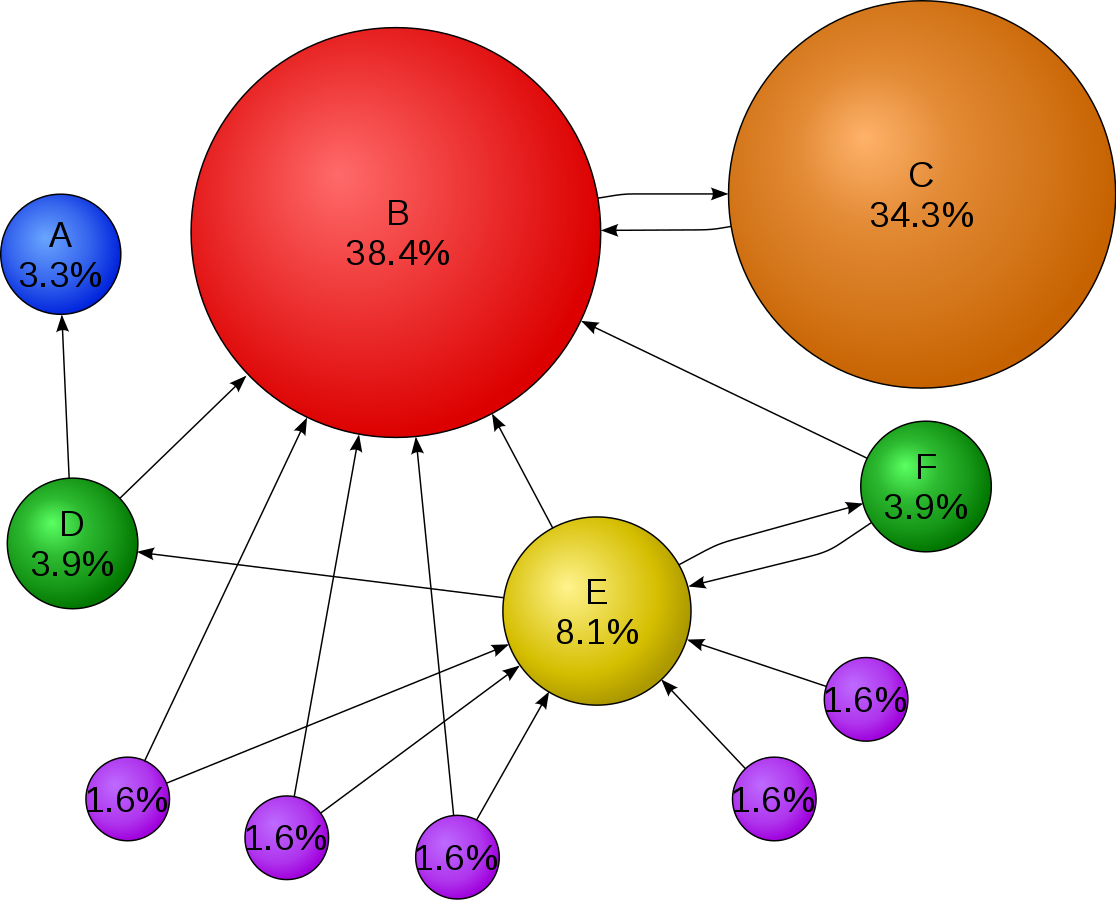
\includegraphics[scale=0.25]{imgs/pagerank-Example.png} 
%\caption{Ilustração de funcionamento do PageRank}
%\label{fig:referencia}
%\end{figure}

%\begin{table}[h!]
%  \begin{center}
%    \caption{Exemplo de tabela (Legenda da Tabela)}
%    \label{tab:tabela1}
%    \begin{tabular}{l|c|r} % <-- Alinhamento: 1 coluna à esquerda, 2 centralizada e 3à direita, com linhas verticais
%      \textbf{Valor 1} & \textbf{Valor 2} & \textbf{Valor 3}\\
%      Vértice & cor & percentual $\gamma$ \\
%      \hline
%      A & azul & $3,3\%$\\
%      B & Vermelho & $38,4\%$\\
%      C & Laranja & $34,3\%$\\
%    \end{tabular}
%  \end{center}
%\end{table}

%-------------------//-----------------------------
\chapter{Referencial Teórico}
\label{chap:referencial}

Neste capítulo, são apresentados os principais conceitos que formam a base teórica do trabalho. 

\section{Equações Diferenciais Ordinárias}

Uma Equação Diferencial Ordinária (EDO) é um tipo de modelo matemático que descreve como as populações modeladas evoluem ao longo do tempo. Os modelos de EDOs são bastante difundidos e utilizados em diversas áreas como, por exemplo, na medicina e na neurociência \cite{ADOMIAN1995107}, no estudo do Câncer \cite{spencer2004ordinary, talkington2018ordinary}, no estudo da resposta imune à infecções virais \cite{reis2021validated}, no estudo da eletrofisiologia cardíaca \cite{VIGMOND20083, bucelli2022mathematical}, entre outros exemplos. 

%A seguir, são apresentados alguns modelos de EDOs clássicos. Esses modelos servem de base para vários outros modelos e possuem características interessantes que são utilizadas em vários modelos.   
A seguir, é apresentado um exemplo de modelo clássico da literatura. 

%\subsection{Modelo predador-presa (Modelo Lotka-Volterra)}

O modelo predador-presa, também conhecido como modelo Lotka-Volterra, modelo a dinâmica da interação entre uma presa e um predador. O modelo é descrito pelas seguintes EDOs: 

\begin{equation}\label{eq:predadorpresa}
    \begin{array}{lr}
    \frac{dH}{dt} = r.H - a.H.P
    \\
    \\
    \frac{dP}{dt} = b.H.P - m.P
    \end{array}
\end{equation}

As populações do modelo e as taxas são: 
\[
    \begin{array}{lr}
    H & \text{Presa}\\
    P & \text{Predador}\\
    r & \text{Taxa de reprodução da presa}\\
    m & \text{Taxa de mortalidade dos predadores}\\
    a & \text{Taxa de predação}\\
    b & \text{Taxa de reprodução dos predadores}\\
    \end{array}.
\]

Neste modelo, temos os seguintes processos sendo modelados: 
\begin{itemize}
    \item Reprodução das presas (termo $r.H$);
    \item Predação (termo $a.H.P$);
    \item Reprodução dos predadores (termo $b.H.P$);
    \item Morte dos predadores (termo $m.P$). 
\end{itemize}

Termos de replicação, predação e morte como os vistos neste modelo são muitos comuns e são empregados na maioria dos modelos. Esses termos são construídos com base no princípio da Lei de Ação de Massas (\textit{Mass Action Law}) que diz que "O número de interações entre duas partículas depende da concentração de ambas". A Lei de Ação de Massas pode ser aplicada, a princípio, a qualquer sistema de qualquer área onde as seguintes hipóteses são consideradas: 
    \begin{itemize}
        \item O sistema é bem homogêneo (\textit{well-mixed system}); 
        \item As partículas/substâncias se movimentam de forma aleatória; 
        \item Não é considerada nenhuma estrutura espacial (\textit{lack of spatial structure}) no modelo.
    \end{itemize}

Na Figura \ref{fig:hostprey}, é dado um exemplo de resultado obtido com a simulação do modelo predador-presa. 

\begin{figure}[h]
    \centering
    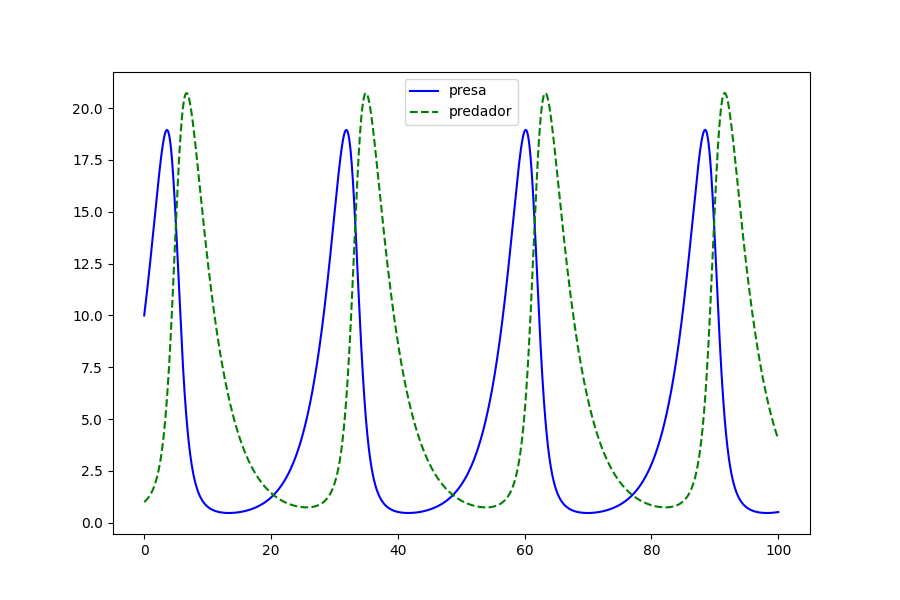
\includegraphics[scale=0.6]{imgs/hostprey.png} 
    \caption{Exemplo de resultado do modelo Predador-Presa clássico.}
    \label{fig:hostprey}
\end{figure}


%\subsection{Modelo da competição entre espécies}

%\subsection{Modelo SIR de transmissão de doenças}

\section{Programação Visual e Editores baseados em Nós}
\label{sec:programacao-visual}

Programação visual é uma maneira do usuário programar a máquina por meio de elementos gráficos que abstraem instruções do computador. Comumente, estes elementos representam múltiplas operações por vez, com o objetivo de facilitar a programação.

Um dos primeiros exemplos da aplicação prática da programação visual foi com a linguagem GRAIL (\textit{GRAphical Input Language}) \cite{grail}, desenvolvida em 1969 junto a um dispositivo semelhante a uma caneta e uma tela sensível ao seu toque. O conjunto do \textit{hardware} e do \textit{software} permitia que o usuário desenhasse letras e formas geométricas que se traduziriam em elementos de fluxograma. O objetivo era realizar um estudo sobre a comunicação humano-computador.

O conceito de utilizar elementos visuais para a assistência da programação não se restringiu somente a dispositivos especializados, contudo, e hoje se encontra em diversos \textit{softwares} de finalidades distintas que podem ser instalados em qualquer computador. Como um exemplo de aplicação de propósito similar ao GRAIL, a linguagem Scratch \cite{scratchlang} foi criada com o objetivo de facilitar o ensino de lógica de programação para crianças sem comprometer em funcionalidades. A linguagem apresenta comandos, funções e estruturas de controle como blocos que podem ser ``montados'' para compor um programa.

Outras aplicações se especializam em algum nicho da computação, como é o caso do simulador lógico Logisim \cite{logisim}, que abstrai componentes lógicos e permite o usuário criar circuitos em uma espécie de \textit{protoboard} digital.

Muitas vezes, \textit{softwares} que incluem programação visual para a abstração de operações utilizam uma interface conhecida como editor de nós:

\begin{itemize}
    \item O \textit{software} de modelagem, animação e edição de vídeos, Blender \cite{blender}, utiliza um editor de nós para abstrair operações de manipulação de imagens e materiais;

    \item O motor de jogos proprietário Unreal Engine\footnote{\href{https://www.unrealengine.com/}{Documentação da Unreal Engine}} utiliza editores de nós para múltiplas finalidades e, entre elas, está a escrita de \textit{shaders} e a programação de lógica geral dos jogos.
\end{itemize}

Existem diversos motivos pelos os quais a programação visual se encontra em tão amplo uso. Principalmente, pode-se atribuir o sucesso de sua aplicação à facilidade de utilização. Em geral, não se faz necessário a leitura de manuais da mesma forma que se faz com linguagens de programação tradicionais; todas as operações possíveis no software estão modeladas como elementos visuais com parâmetros de entrada e saída bem definidos. Implementações exemplares também proibirão o usuário de realizar ligações inválidas diretamente na interface, realizando uma etapa mais comum em compiladores ou analizadores estáticos de código, que geralmente permitem que o usuário cometa um ou mais erros e só descubra-os posteriormente.

\section{Geração de código}

A fase de geração de código geralmente é a última fase da compilação. Na maioria dos compiladores, o gerador de código recebe como entrada uma ou mais representações intermediárias do código/texto de entrada e retorna como saída o código/texto na linguagem alvo \cite{dragonBook}. 

Como este trabalho tem o objetivo de possibilitar a geração de código em múltiplas linguagens alvo diferentes, surgiu a necessidade de abstrair mais esta fase, de forma que a implementação de linguagens alvo adicionais seja mais simples dado que ao menos uma já foi implementada.

Para tal abstração, seguiu-se um padrão utilizado por diversos compiladores diferentes, que consiste na separação do \textit{back-end} (que trabalha com a linguagem alvo) do \textit{front-end} (que trabalha com a linguagem fonte) através da utilização de uma ou mais representações intermediárias. 

Nas próximas subseções, serão apresentados alguns conceitos importantes para o entendimento do processo de geração de código. 

\subsection{Representação intermediária}

As representações intermediárias (RIs) são usadas em um compilador por várias razões \cite{dragonBook}, dentre as quais destaca-se: 
\begin{itemize}
    \item Separar o \textit{front-end} do \textit{back-end}. Neste caso, o \textit{front-end} não precisa se preocupar com detalhes da linguagem alvo e o \textit{back-end} não precisa conhecer detalhes da linguagem fonte;
    \item Permitir que sejam realizadas otimizações independente de máquina ou otimizações independente da linguagem alvo; 
    \item Para facilitar a tradução e geração do código alvo.    
\end{itemize}

Algumas RIs usadas em compiladores incluem:  
\begin{itemize}
    \item Árvore de Sintaxe Abstrata (ASA); 
    \item Grafos Acíclicos Dirigidos (GAD); 
    \item Código de Três Endereços. 
\end{itemize}

As Árvores de Sintaxe Abstratas são muito usadas na representação do código fonte de entrada, representando comandos e expressões em cada escopo. Os Grafos Acíclicos Dirigidos são muito usados na fase de otimização do código. O Código de Três Endereços é uma representação que está próxima da linguagem Assembly e pode ser usada como base para várias otimizações independentes da máquina. Geralmente, o Código de Três Endereços otimizado é a entrada recebida pelo gerador de código Assembly. O Código de Três Endereços também pode ser utilizado pelo algoritmo de alocação de registradores como uma abstração inicial para a escolha e atribuição de registradores.    

%TODO: Falar da representação intermediária do LLVM e a sua importância no desenvolvimento de compiladores que utilizam o back-end do LLVM para gerar código para várias arquiteturas. 

Como uma alternativa mais abstrata ao Assembly (que é dependente da arquitetura alvo), existe a linguagem LLVM IR (LLVM \textit{Intermediate Representation}), que por sua vez pode ser transpilada para o Assembly da máquina alvo. A LLVM é uma infraestrutura para o desenvolvimento de compiladores com o objetivo de facilitar sua criação sem se preocupar com a arquitetura de computadores. Considerando que uma linguagem possa ser transpilada na representação intermediária da LLVM (LLVM IR), ela pode ser compilada em qualquer arquitetura suportada pela infraestrutura que incluem, mas não estão limitadas a, x86, AMD64, ARM, ARM64, WebAssembly e RISC-V.

Para facilitar o processo de geração de código e realizar uma maior separação entre o \textit{front-end} (interface gráfica) e o \textit{back-end} (gerador de código) do software, foi criada e utilizada uma representação intermediária (RI). A RI é a entrada para o gerador de código e também é utilizada para salvar e carregar os modelos. A RI desenvolvida será apresentada e explicada na Seção \ref{subsection:RI}.

\subsection{Sistemas baseados em \textit{templates}}
 
Em várias aplicações, a geração de código é feita com base em \textit{templates}. Desde o início da World Wide Web, \textit{templates} têm sido usados por \textit{frameworks} para ajudar no processo de construção de páginas Web. Informalmente, podemos dizer que um \textit{template} é um esqueleto (uma estrutura) que serve de referência para todo o processo de geração de código.

Em sua essência, \textit{templates} são arquivos com marcadores especiais que podem ser substituídos por outros valores dinamicamente, de forma similar ao pré-processador de C. Adicionalmente, alguns motores de \textit{templates} introduzem estruturas de controle de fluxo, como condicionais, laços de repetição e chamadas de funções. 

Para ilustrar a ideia, suponha o \textit{template} abaixo criado com base em um código que implementa um sistema de Equações Diferenciais Ordinárias (EDOs):  

\begin{lstlisting}[language=Python, firstnumber=1]
from scipy.integrate import solve_ivp
import numpy as np
import pandas as pd

def odeSystem(t, P,  {{key}}  {{key}}, ):
## for key, value in vars
    {{key}} = P[{{loop.index}}]
## endfor
## for key, value in odes
    d{{key}}_dt = {{value}}
## endfor     
    return  [ d{{key}}_dt  d{{key}}_dt, ]
\end{lstlisting}

O \textit{template} acima utiliza os marcadores definidos pela biblioteca Inja\footnote{\href{https://github.com/pantor/inja}{https://github.com/pantor/inja}}, e demonstra algumas das estruturas de controle mencionadas, na forma das palavras-chave \texttt{\textcolor{codepurple}{for}}, \texttt{\textcolor{codepurple}{if}} e \texttt{\textcolor{codepurple}{else}}.

%\section{Simulação computacional}

%Chama-se de simulação computacional o processo dinâmico de instanciar um modelo, seja este tradicional (expressado por equações) ou mais abstrato (expressado por objetos, agentes, operadores ou algoritmos), como definido em \cite{compsim}. 

%Estas simulações possibilitam a existência diversos serviços que hoje são essenciais para os seres humanos, como previsão do tempo (), construção de aviões aero-dinâmicos () e estudos de epidemias ().

%As simulações computacionais também permitem a avaliação de diferentes cenários em pouco tempo. Para as EDOs, isto possibilita a compreensão do efeito que cada componente tem no resultado final.

% Simulação computacional: 
% 	- O que é?
% 	- Qual a sua importância?
% Simulação de cenários: 
% 	Uma abordagem baseada em cenários se mostra interessante porque através desses diferentes cenários é possível compreender melhor como cada célula/substância do modelo interage e como os comportamentos emergem a partir dessas interações. Outra característica importante é a possibilidade de se analisar os efeitos de remover determinada célula/substância do modelo. 

\section{Ensino-aprendizagem de Modelagem Computacional} %TODO

%Falar sobre Metodologias ativas, aprendizagem baseada em problemas/projetos (Problem based learning) 

Os modelos são abstrações do mundo real. Com a evolução dos computadores e o seu uso massivo, os modelos computacionais têm contribuído significativamente para o avanço do conhecimento em diversas áreas. Eles nos ajudam a compreender os fenômenos de interesse permitindo “rastrear” e entender as mudanças que estão ocorrendo em um sistema complexo e visualizar, por exemplo, o efeito de uma pequena mudança no restante do sistema. 

Simulações computacionais são ferramentas fundamentais não só para a pesquisa científica, mas também para a educação. Elas são frequentemente usadas como laboratórios virtuais para promover a compreensão dos alunos sobre os conceitos teóricos que estão na base dos sistemas simulados. [Imagining the School of the Future Through Computational Simulations: Scenarios’ Sustainability and Agency as Keywords]. 

Após a Segunda Guerra Mundial, o leque de campos disciplinares em que as simulações começaram a ser utilizadas tem vindo a expandir-se até os dias de hoje, de modo que é quase impossível nomear qualquer disciplina que não tenha utilizado ou desenvolvido ferramentas computacionais e simulações para avançar a fronteira do conhecimento (Borrelli e Wellmann, 2019).

O uso de modelos computacionais abre novas maneiras para os alunos aprenderem sobre diferentes disciplinas. Os alunos podem aprender através de um processo iterativo de construção de modelo, simulação, modificação de modelo para simulação novamente, explorando todas as características do modelo em si [Imagining the School of the Future Through Computational Simulations: Scenarios’ Sustainability and Agency as Keywords]. Plataformas como, por exemplo, a Netlogo [ref] permitem este tipo de aprendizagem iterativa e interativa.

Um dos objetivos do software que foi desenvolvido neste trabalho é auxiliar o aprendizado de conceitos importantes nas áreas de modelagem matemática e computacional e ajudar o aluno a desenvolver a habilidade de modelar problemas através da prática de construção e simulação de modelos. O uso combinado do software com alguma metodologia ativa de ensino permitirá aos alunos aprender na prática como construir modelos para diferentes fenômenos de interesse e entender melhor os fenômenos estudados através das simulações computacionais realizadas de forma interativa através da interface gráfica do software. 

Considerando o uso do software na prática e uma visão geral do chamado ciclo da modelagem apresentado na Figura …, destaca-se que o software auxilia o passo 2 e automatiza os passos 3 e 4 facilitando o processo de modelagem por estudantes e pesquisadores. 

%TODO: Fazer figura do ciclo com os passos abaixo 

1) Estudo do problema.
2) Formulação do modelo.
3) Implementação do modelo.
4) Simulação computacional.
5) Validação do modelo.

O aprendizado, em sala de aula, pode ser conduzido, por exemplo, através de um processo incremental que começa investigando e trabalhando com modelos mais simples até se chegar em modelos mais complexos. Algumas vantagens incluem:  1) a apresentação de determinados conceitos e técnicas é facilitada em modelos mais simples; 2) em muitos casos reais, modelos complexos utilizam certas expressões, equações e “estratégias” na modelagem que estão presentes também em modelos mais simples. Então, muitas vezes, o aluno conseguirá entender melhor um modelo mais complexo entendendo que determinadas partes do mesmo já apareceram em modelos mais simples previamente estudados. 

Uma possível abordagem de ensino seria o professor trabalhar com um problema para apresentar e discutir alguns conceitos e/ou técnicas de modelagem de forma semelhante à metodologia Problem Based Learning (PBL) [refs]. O seguinte conjunto de passos é sugerido a seguir: 

\begin{enumerate}
 \item Descrição do contexto e do problema a ser modelado;
 \item Formulação das hipóteses pelos alunos e discussão entre eles;
 \item Formulação do modelo considerando o conhecimento de modelos existentes e que foram estudados previamente;
 \item Construção do modelo no software;
 \item Simulação do modelo no software com a criação de diferentes cenários para teste e análise dos comportamentos obtidos.
 \item Caso o comportamento desejado ou esperado não seja obtido, voltar para o passo 2.
\end{enumerate}

As metodologias ativas de ensino colocam o aluno como protagonista no processo de construção do próprio conhecimento. ... 

%---------------------------------//-----------------------------
\chapter{Trabalhos relacionados}
\label{chap:relacionados}

Com o avanço de tecnologias para o desenvolvimento de aplicações gráficas e também da internet, ocorreu um aumento expressivo na quantidade de \textit{softwares} desenvolvidos para modelagem e simulação computacional. Entrentanto, poucos destes \textit{softwares} permitem que o usuário visualize e interaja com o código gerado para a simulação de seu modelo. Mais comumente, a única maneira com a qual o usuário pode interagir com o modelo é através da abstração provida pela interface, o que causa uma dependência direta do \textit{software}.

%TODO
A seguir, na Tabela ... é apresentado um quadro comparativo entre o software deste trabalho e softwares similares. Para realizar a comparação, foram selecionadas algumas características consideradas relevantes no contexto de softwares para modelagem e simulação computacional. 

%TODO: TABELA (Quadro comparativo)

O software desenvolvido possui alguns diferencias em relação a outros desenvolvidos com propósitos similares:

\begin{itemize}
    \item Em sua interface gráfica é apresentado um editor baseado em nós que fornece ao usuário uma forma de programação visual \ref{sec:programacao-visual}, possibilitando um grau de liberdade limitando apenas operações consideradas incorretas;
    
    \item Em seu formato de representação intermediária para salvamento e carregamento dos modelos, o software utiliza uma estrutura extensível para outros tipos de modelos como, por exemplo, equações diferenciais parciais. Esta estrutura também foi projetada para ser humanamente legível, a ponto de ser possível que uma pessoa decodifique o modelo representado apenas lendo o arquivo. Assim, caso o software se prove insuficiente ou indisponível, ainda é possível reverter o arquivo nas equações que o compõe. % TODO: Este parágrafo fez sentido? Fez sentido para mim. Ficou muito bom.  
\end{itemize}

A seguir, são descritos em mais detalhes os trabalhos relacionados. 

\section{Snoopy}

Um \textit{software} que serviu como inspiração para este trabalho foi o software para construção, animação e simulação de redes de Petri chamado Snoopy \cite{Heiner2008,Heiner2012,Liu2012}. Além da rede de Petri clássica, o software permite modelar e simular vários tipos de redes de Petri como, por exemplo, redes de Petri estocásticas e coloridas que são extensões da rede clássica. O modelo construído é representado como um grafo que tem dois tipos de nós chamados \textit{places} (locais) e \textit{transitions} (transições) e quatro tipos de arestas (estocástica, imediata, determinística e planejada) com suas semânticas associadas. Os \textit{places} representam populações de um certo tipo e transições representam eventos que podem aumentar ou diminuir as quantidades das populações que estão armazenadas nos locais. 

O modelo gráfico utilizado pelo software Snoopy serviu de inspiração para a criação da representação utilizada neste trabalho. A partir do software Snoopy, foi possível observar que modelos gráficos, além do atrativo visual, facilitam a construção de um modelo e um melhor entendimento do que está sendo feito, o que está sendo modelado. A possibilidade de simular interativamente as Redes de Petri estocásticas foi um fato que serviu de inspiração para a ideia da simulação interativa no software desenvolvido neste trabalho. 

\section{Insight maker}
    
O InsightMaker \cite{insightmaker} é um \textit{software} de simulação baseado em nuvem. Todo o modelo é feito através de um navegador de internet e, quando executado, é simulado no próprio servidor, sem a necessidade de que o usuário possua uma máquina potente. O InsightMaker \cite{insightmaker} permite a construção de modelos utilizando diagramas de Dinâmica de Sistemas e modelos baseados em agentes. O site possui diversas facilidades para a construção do modelo em um Canvas. A partir do modelo de Dinâmica de Sistemas construído no Canvas, o InsightMaker \cite{insightmaker} gera internamente um modelo de EDOs e executa este modelo utilizando o método de Euler ou o método de Runge-Kutta de quarta ordem conforme escolha do usuário. Através da interface web, também é possível definir os valores de todas as variáveis e parâmetros, e é possível realizar as simulações computacionais. Os resultados são exibidos de forma interativa onde é possível controlar a velocidade com que os valores são exibidos nos gráficos. 

\section{VCell}

O software VCell (Virtual Cell) \cite{vcell,VCellref1} é uma plataforma para modelar sistemas biológicos celulares que é construída em torno de um banco de dados central e disseminada como um aplicativo da web. Os modelos são construídos com base em regras (\textit{Rule-based modelling}). VCell tem os seguintes tipos de simulações disponíveis: determinística (EDO compartimental ou EDP de reação-difusão-advecção com suporte para cinemática 2D), reações estocásticas (solvers de SSA), estocástica espacial (reação-difusão com Smoldyn), híbrida determinística/estocástica e simulações baseadas em agentes. O software permite simular vários processos metabólicos que ocorre dentro das células e através das membranas celulares. Com relação às membranas, há suporte para os seguintes processos: Eletrofisiologia, suporte para o fluxo da membrana e difusão lateral da membrana. 

\section{EpiFire}

O EpiFire \cite{epifire} não é um \textit{software} completo, mas uma biblioteca em C++ para simulação de modelos de redes complexas com aplicação na área de Epidemiologia. Ele é uma interface de programação de aplicativos (API) implementado em C++, projetado para gerar de forma eficiente redes com uma distribuição de grau especificada, medir características fundamentais da rede e realizar simulações computacionais eficientes das redes geradas com base nos métodos \textit{percolation} e \textit{chain-binomial}. 

\section{Cytoscape}

O software Cytoscape \cite{shannon2003cytoscape} é uma plataforma de software de código aberto para visualizar redes de interação molecular e vias biológicas e integrar essas redes com anotações, perfis de expressão gênica e outros dados. Atualmente, o Cytoscape é utilizado como uma plataforma geral para análise e visualização de redes complexas. 

%OpenFOAM (https://www.openfoam.com/)
%Stella (https://www.iseesystems.com/store/products/stella-online.aspx)


\chapter{Software para modelagem e simulação computacional}
\label{chap:metodologia}
\label{chap:software-para-modelagem}

O \textit{software} desenvolvido neste trabalho consiste em uma interface gráfica de usuário \ref{fig:gui-predador-presa} (mais comumente referida pelo acrônimo em inglês, GUI, que significa \textit{Graphical User Interface}) que apresenta um editor baseado em nós. Os nós representam abstrações de componentes comumente usados na construção de EDOs, como constantes, variáveis e expressões matemáticas. Na Seção \ref{sec:representacao-visual-edo}, serão apresentados os tipos de nós presentes na interface.

\begin{figure}[h]
    \centering
    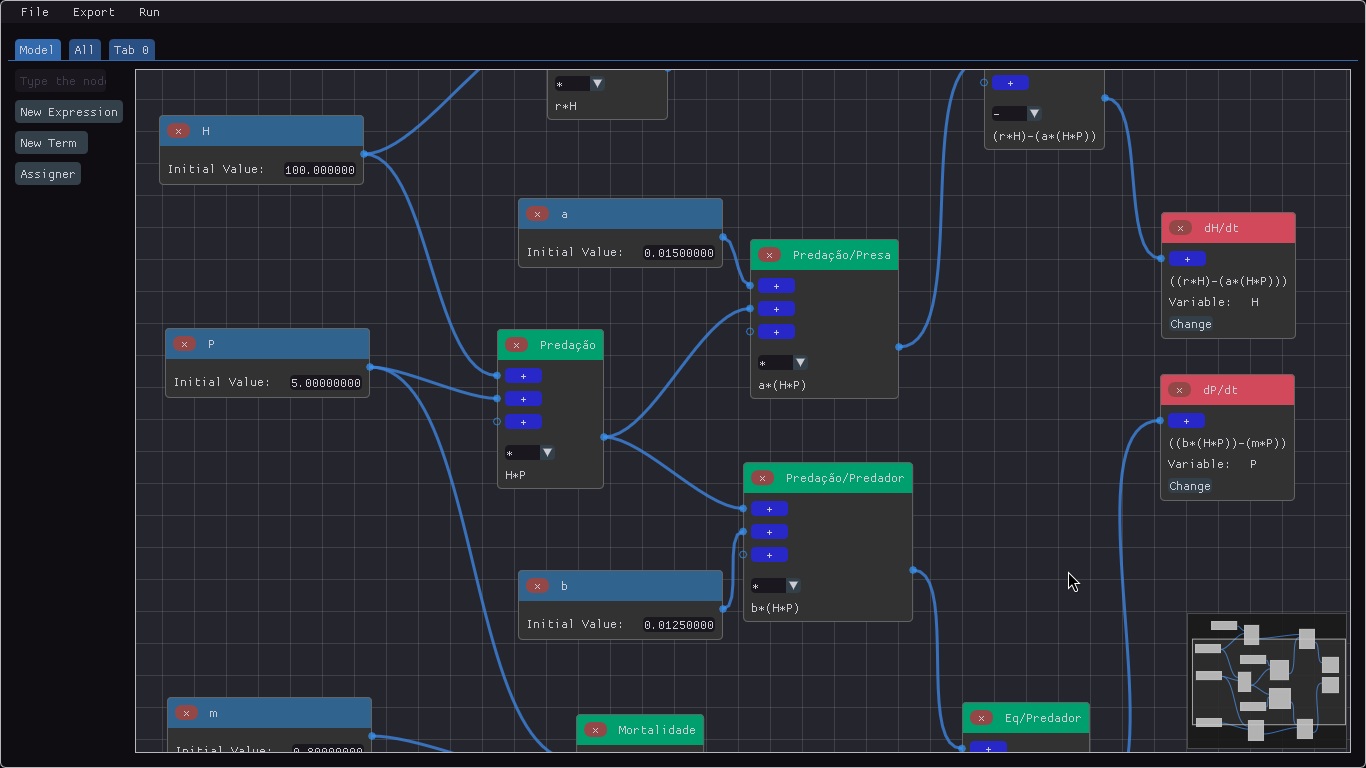
\includegraphics[scale=0.35]{imgs/ode-designer/predador-presa.png} 
    \caption{Exemplo do modelo Predador-Presa (\ref{eq:predadorpresa}) construído no \textit{software}.}
    \label{fig:gui-predador-presa}
\end{figure}

Após construído o modelo, o usuário poderá simulá-lo diretamente pela GUI \ref{fig:gui-grafico-all}, exportar um PDF dos resultados, ou exportar um código de Python que implementa computacionalmente o modelo desenhado \ref{code:predador-presa}. A experiência de usuário pode ser resumida ao fluxograma \ref{fig::experiencia_usuario}.

\begin{figure}[h]
    \centering
    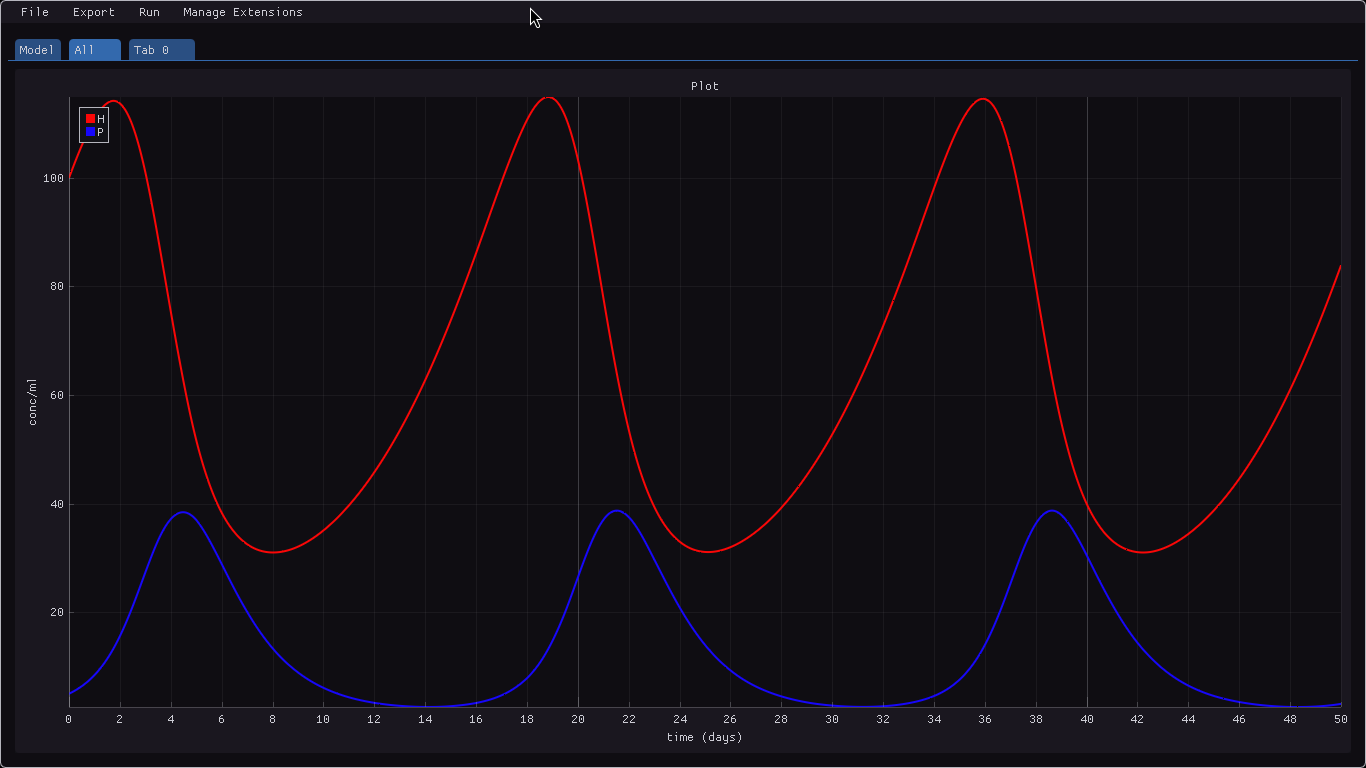
\includegraphics[scale=0.35]{imgs/ode-designer/grafico-all.png} 
    \caption{Plotagem dos resultados da simulação do modelo Predador-Presa.}
    \label{fig:gui-grafico-all}
\end{figure}

\begin{figure}[h]
    \centering
    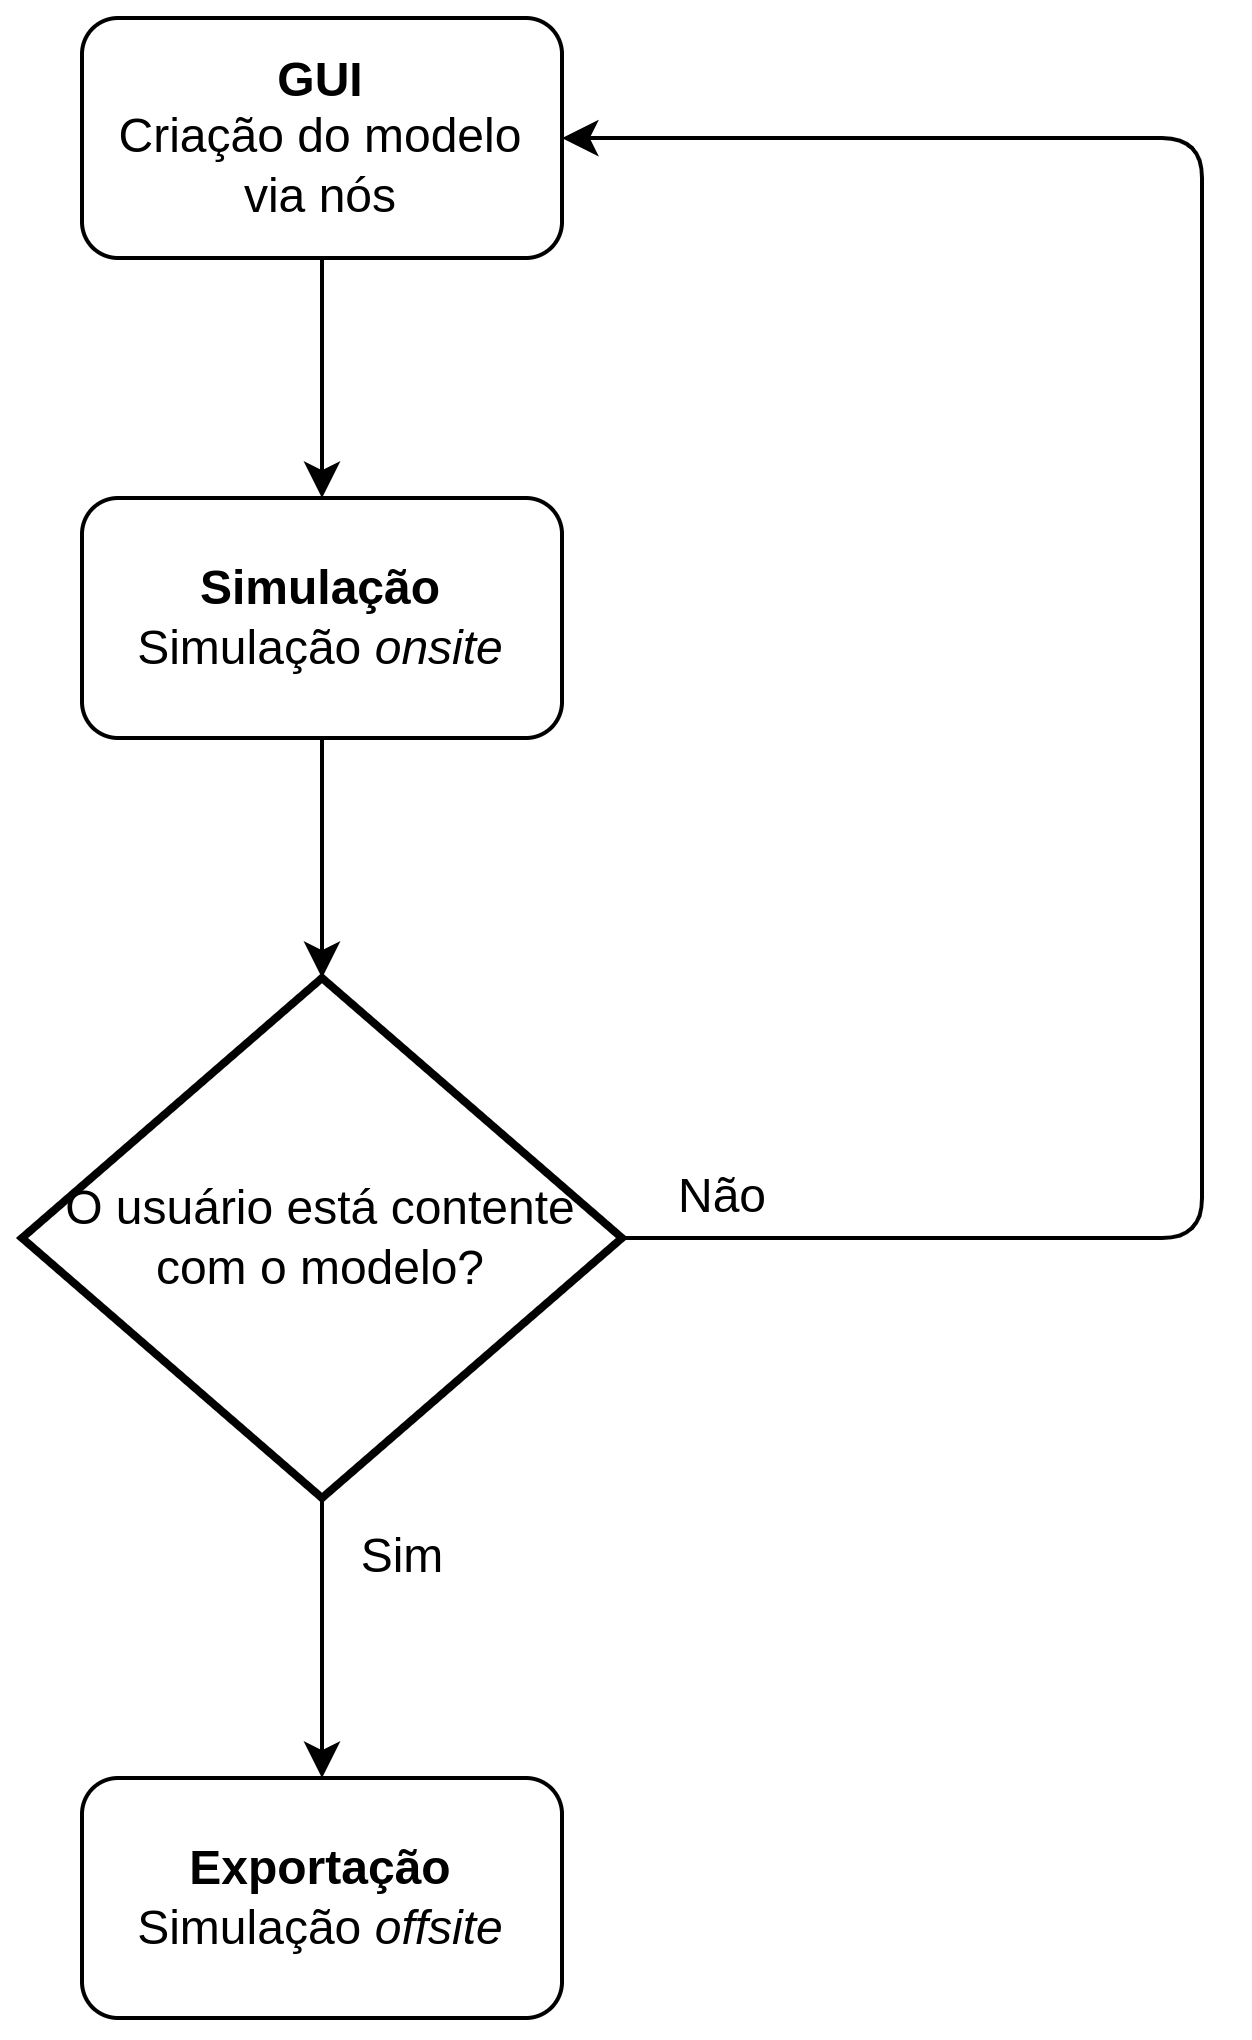
\includegraphics[scale=0.25]{imgs/fluxograma.png} 
    \caption{Fluxograma da experiência de usuário esperada para o software.}
    \label{fig::experiencia_usuario}
\end{figure}

Dessa forma, o usuário pode criar e simular modelos sem a necessidade de iniciar a implementação computacional do zero e também sem a necessidade de ter muito conhecimento dos métodos que são utilizados na implementação. O usuário terá acesso aos códigos gerados e poderá utilizá-los, por exemplo, como base para desenvolver o seu próprio código. 

A simulação das EDOs, tanto pela GUI quanto pelo código de Python exportado, é feita utilizando métodos especializados da biblioteca ciêntífica \texttt{scipy} \cite{scipy}. % Devemos entrar em detalhes de como isso é feito? Se sim, precisamos de uma explicação do método RK45

\section{Arquitetura do software}

\begin{figure}[h]
    \centering
    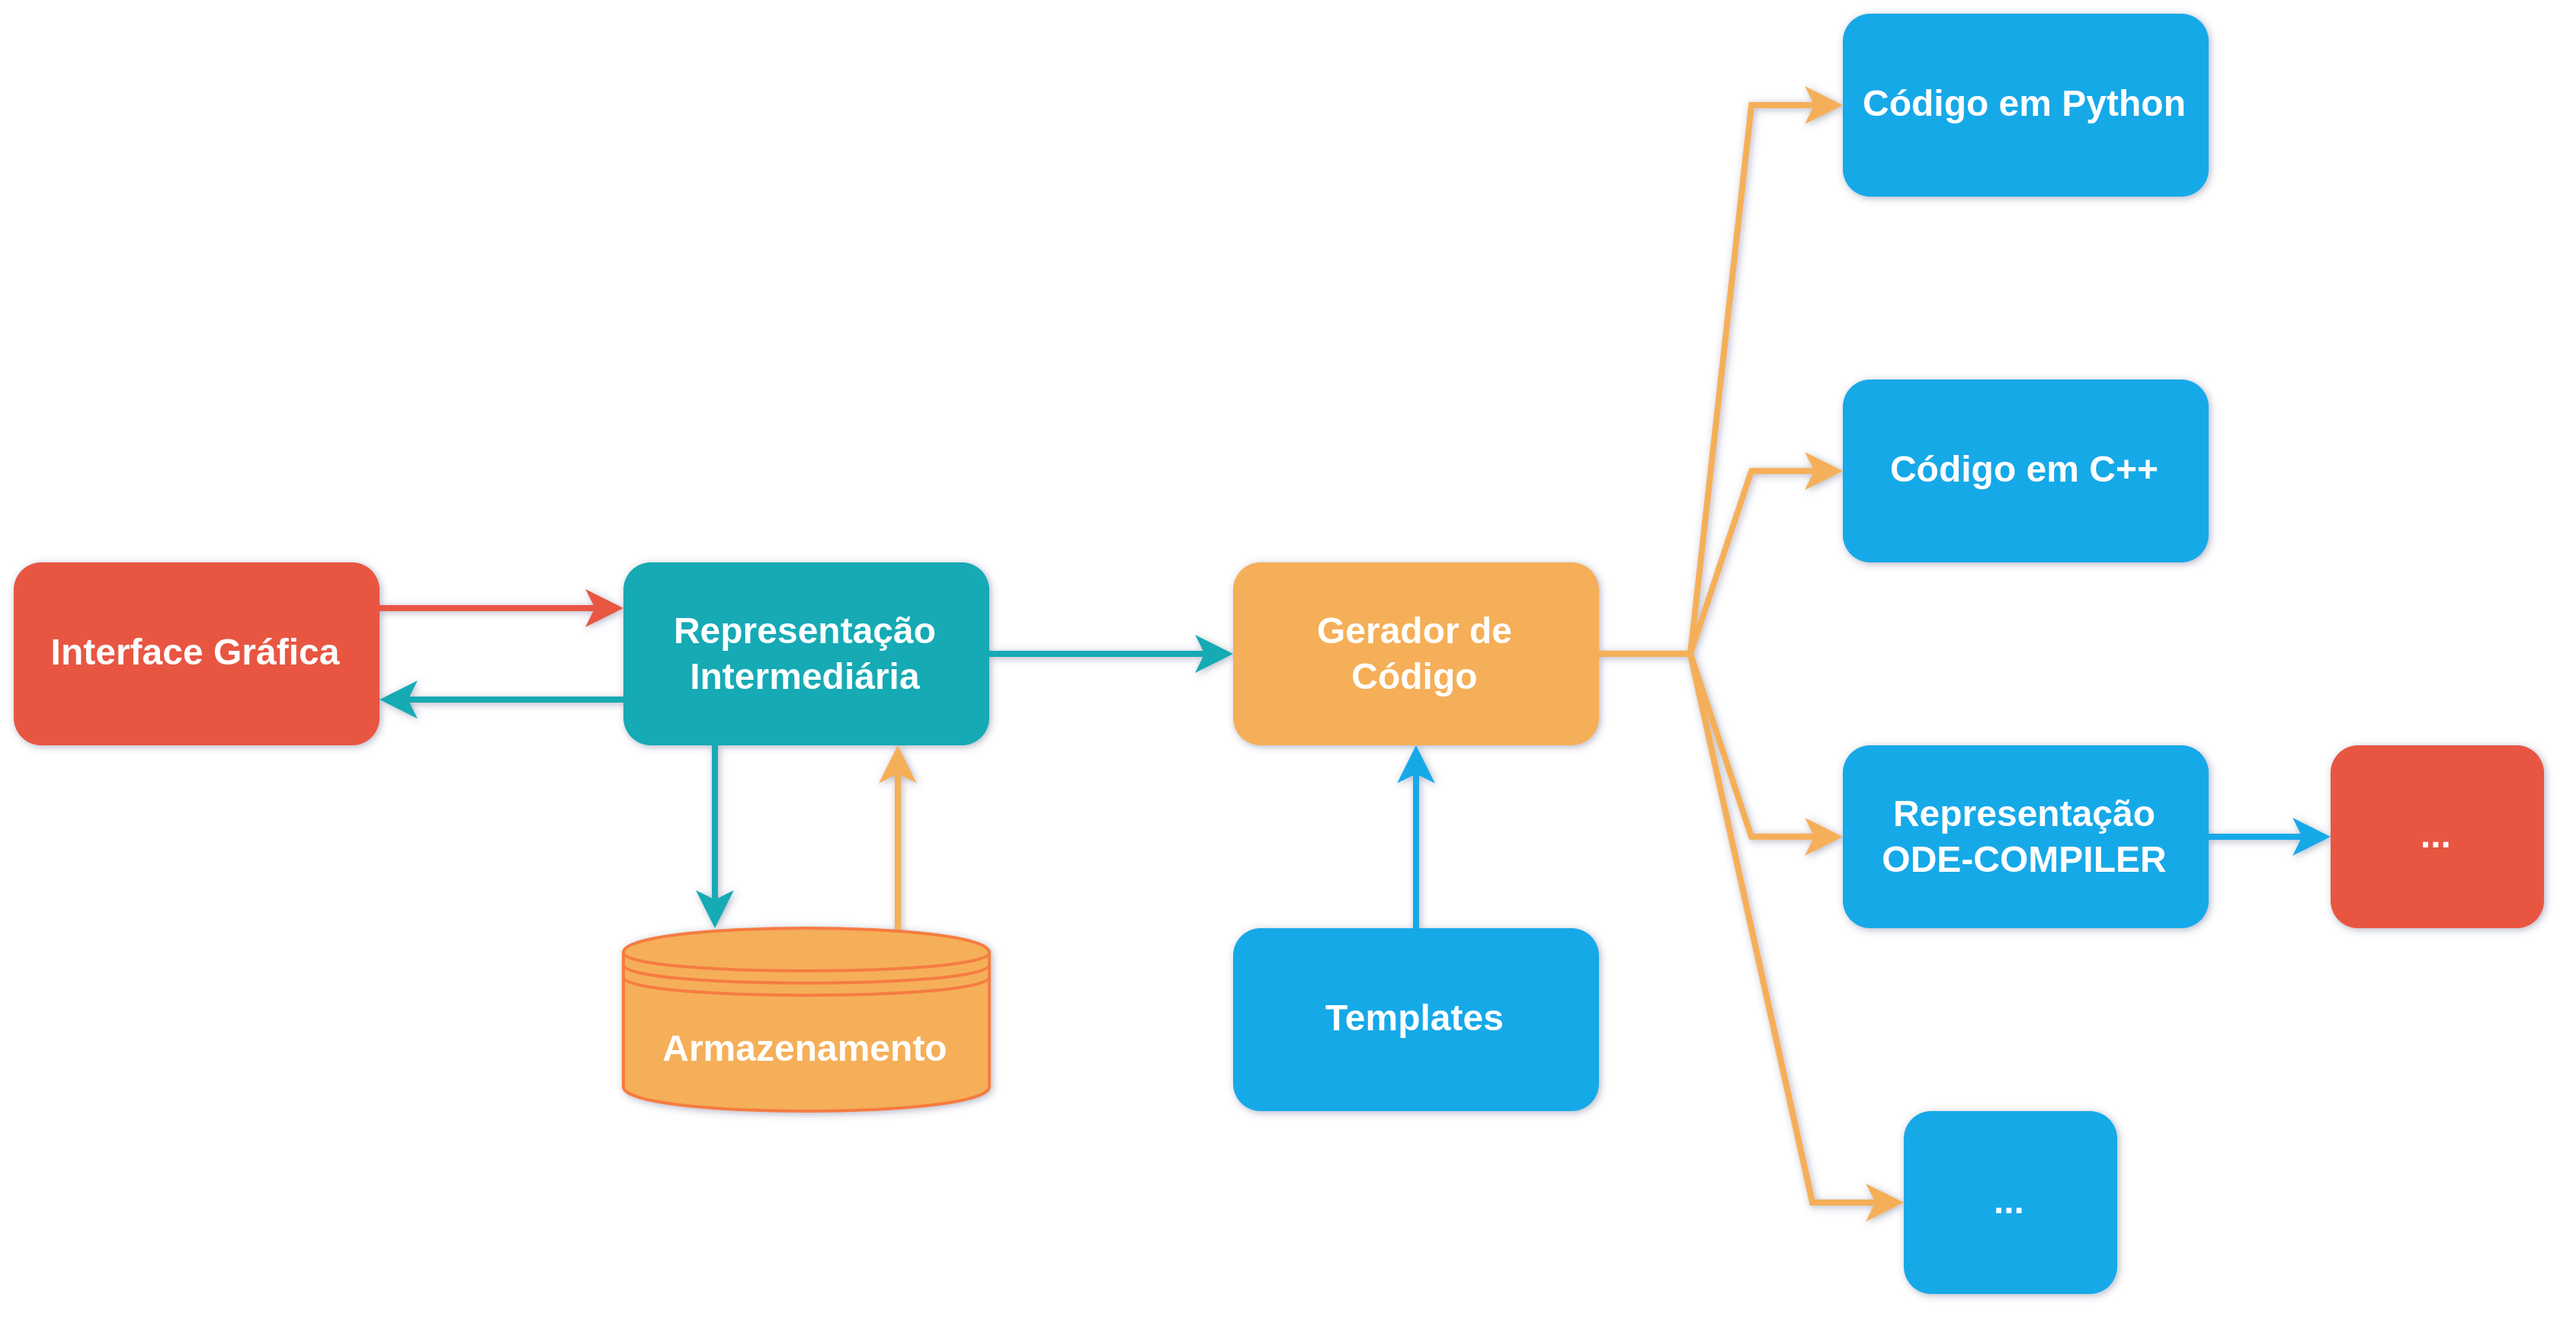
\includegraphics[scale=0.125]{imgs/passos_divisao_software.png} 
    \caption{Visão arquitetural do software.}
    \label{fig::arquitetura_software}
\end{figure}

Na Figura \ref{fig::arquitetura_software}, é apresentada uma visão geral do software onde são destacados os módulos principais, suas interações e suas entradas e saídas. A \textbf{Interface Gráfica} é o módulo que implementa toda a parte visual do software através da qual o usuário interagirá. Este módulo pode ter seus dados transformados de e para a \textbf{Representação Intermediária} (RI), que será explicada na Seção \ref{subsection:RI}. Por meio desta, o software pode salvar e carregar os dados da interface no computador, além de ser a entrada para o \textbf{Gerador de Código} baseado em \textbf{\textit{Templates}}.

O gerador de código irá injetar os dados disponíveis na RI em pontos específicos do \textit{template} para gerar o código que implementa o modelo computacionalmente. Por exemplo, caso o usuário deseje gerar o o código em Python, o \textit{template} correspondente será carregado e terá seus marcadores substituídos por trechos específicos da RI. Destaca-se que a ferramenta poderá ser estendida e modificada para gerar código para mais linguagens ou até códigos/arquivos que são entrada para outros simuladores. 

%TO DO: diagrama com os principais módulos do software e falar no texto das estruturas de cada módulo 

%    pub labels: Vec<String>,
%    pub lines: Vec<Vec<f64>>,
%    pub time: Vec<f64>,
%    pub title: String,
%    pub xlabel: String,
%    pub ylabel: String,
%    pub data: CSVData,
%Falar por alto das estruturas que armazenam as informações do plot 
%Os resultados da simulação e os metadados são armazenadas em estruturas específicas que servem de entrada para a plotagem do gráfico. 
% 
%A interface gráfica será capaz de realizar duas plotagens diferentes. A primeira será feita em tempo real levando em consideração as alterações do usuário. 

A plotagem dos resultados da simulação é feita utilizando a biblioteca \textbf{ImPlot}\footnote{\href{https://github.com/epezent/implot}{https://github.com/epezent/implot}}.

\section{Uma representação visual para EDOs}
\label{sec:representacao-visual-edo}

\subsection{Representação intermediária}\label{subsection:RI}

Neste trabalho, a representação intermediária (RI) foi utilizada com dois propósitos: (1) Separar o \textit{front-end} (interface gráfica) do \textit{back-end} (gerador de código) e (2) Permitir que os modelos construídos sejam salvos e carregados da unidade de armazenamento.

A RI evita que mudanças realizadas no código da interface gráfica tenham um grande impacto na implementação do gerador de código. Desta forma, o gerador de código somente será impactado por alguma mudança na \textit{GUI} quando a mudança tiver como efeito a inserção, modificação ou remoção de informações da representação intermediária.

A alternativa a esta abordagem seria passar as informações em memória do modelo diretamente para o gerador de código. Neste caso, o acoplamento dos módulos seria maior, e o impacto disto seria maior tempo de desenvolvimento para cada nova transformação adicionada (por exemplo, novas linguagens de programação).

Para permitir que o usuário salve e carregue os modelos, a RI assumida se baseia num formato JSON que representa de forma direta as classes de C++ que formam a GUI. Para a serialização e deserialização em JSON, utilizou-se uma biblioteca da linguagem Rust chamada \textit{serde} (que será explicada em detalhes na Seção \ref{sec:tecnologias}), que permite que esta conversão seja feita de forma declarativa. Na listagem a seguir, é mostrado um exemplo de arquivo JSON que é referente ao modelo Predador-Presa (Figura \ref{fig::exemplo_gui}). As EDOs desse modelo foram apresentadas na Equação \ref{eq:predadorpresa}. 

%TO DO: Colocar a RI com os dados do modelo predador-presa 

\colorlet{punct}{red!60!black}
\definecolor{background}{HTML}{EEEEEE}
\definecolor{delim}{RGB}{20,105,176}
\colorlet{numb}{magenta!60!black}

\lstdefinelanguage{json}{
    basicstyle=\normalfont\ttfamily,
    numbers=left,
    numberstyle=\scriptsize,
    stepnumber=1,
    numbersep=8pt,
    showstringspaces=false,
    breaklines=true,
    frame=lines,
    backgroundcolor=\color{background},
    literate=
     *{0}{{{\color{numb}0}}}{1}
      {1}{{{\color{numb}1}}}{1}
      {2}{{{\color{numb}2}}}{1}
      {3}{{{\color{numb}3}}}{1}
      {4}{{{\color{numb}4}}}{1}
      {5}{{{\color{numb}5}}}{1}
      {6}{{{\color{numb}6}}}{1}
      {7}{{{\color{numb}7}}}{1}
      {8}{{{\color{numb}8}}}{1}
      {9}{{{\color{numb}9}}}{1}
      {:}{{{\color{punct}{:}}}}{1}
      {,}{{{\color{punct}{,}}}}{1}
      {\{}{{{\color{delim}{\{}}}}{1}
      {\}}{{{\color{delim}{\}}}}}{1}
      {[}{{{\color{delim}{[}}}}{1}
      {]}{{{\color{delim}{]}}}}{1},
}

\begin{lstlisting}[language=json]
{
    "meta_data": {
        "start_time": 0,
        "end_time": 10.50,
        "delta_time": 0.1
    },
    "nodes": {
        "1": {
            "id": 1,
            "name": "Population 1",
            "related_constant_name": "Population 1_0",
            "links": [
                {
                    "sign": "+",
                    "node_id": 30
                }
            ],
        },
        "2": {
            "id": 2,
            "name": "Population 2",
            "related_constant_name": "Population 2_0"
        },
        "30": {
            "id": 30,
            "name": "Pop1 + Pop2",
            "operation": "+",
            "inputs": [1, 2]
        }
    }, 
    "constants": [
        {
            "name": "gravity",
            "value": 9.81
        },
        {
            "name": "Population 1_0",
            "value": 100
        },
        {
            "name": "Population 2_0",
            "value": 100
        },
        {
            "name": "a",
            "value": 1.6
        }
    ]
}
\end{lstlisting}

Neste exemplo de RI, pode-se observar 3 seções:

\begin{itemize}
    \item \texttt{"meta\_data"}: Esta seção inclui os meta dados da simulação que não fazem parte de nenhuma construção específica. Entre estes dados, estão o tempo inicial da simulação (\texttt{"start\_time"}), tempo final (\texttt{"end\_time"}) e o passo de tempo (\texttt{"delta\_time"});

    \item \texttt{"nodes"}: Esta seção inclui os nós como vistos interface gráfica. Estes nós podem ser do tipo ``população'' ou ``combinação''.
    
    No primeiro caso, o nó define as relações que ele possui com outros nós pelo atributo \texttt{"links"}. As ligações possuem os dados de sinal (se a relação é positiva (+) ou negativa (-) para a população) e o identificador do nó combinatório relacionado.

    No segundo caso, o nó define o atributo \texttt{"inputs"}, que é uma lista dos identificadores dos nós que se ligam a este. Diferentemente do sub-atributo \texttt{"node\_id"} do nó anterior, estes identificadores podem ser de qualquer tipo de nó.

    A partir desta estrutura, é possível montar as equações de qualquer população através de uma resolução recursiva de identificadores. Em \ref{code::equation-template-jinja} é apresentado um \textit{template} na linguagem Jinja2\footnote{\href{https://jinja.palletsprojects.com/en/3.1.x/}{Jinja2 Homepage}} capaz de realizar a construção das equações como descrito;

    \item \texttt{"constants"}: Esta seção inclui as constantes que podem ser utilizadas em equações, com seus nomes e valores.
\end{itemize}

\definecolor{template_brackes}{HTML}{0431FA}
\definecolor{template_keyword}{HTML}{859900}
\definecolor{template_magic_variable}{HTML}{268BD2}

\lstdefinelanguage{jinja2}{
    basicstyle=\normalfont\ttfamily,
    numbers=left,
    numberstyle=\scriptsize,
    stepnumber=1,
    numbersep=8pt,
    showstringspaces=false,
    breaklines=true,
    frame=lines,
    backgroundcolor=\color{background},
    literate=
     *{\{}{{{\color{template_brackes}\{}}}{1}
      {\}}{{{\color{template_brackes}\}}}}{1}
      {(}{{{\color{template_brackes}(}}}{1}
      {)}{{{\color{template_brackes})}}}{1}
      {\%}{{{\color{template_brackes}\%}}}{1}
      {loop}{{{\color{template_magic_variable}loop}}}{4}
      {recursive}{{{\color{template_keyword}recursive}}}{9}
      {if}{{{\color{template_keyword}if}}}{2}
      {else}{{{\color{template_keyword}else}}}{4}
      {for}{{{\color{template_keyword}for}}}{3}
      {endif}{{{\color{template_keyword}endif}}}{5}
      {endfor}{{{\color{template_keyword}endfor}}}{6}
      {set}{{{\color{template_keyword}set}}}{3}
      {not}{{{\color{template_keyword}not}}}{3}
      {[}{{{\color{delim}{[}}}}{1}
      {]}{{{\color{delim}{]}}}}{1},
}

\begin{lstlisting}[language=jinja2, label={code::equation-template-jinja}][H]
Equations:

 
  - d{{ node.name }}/dt =
  
   
   
    ({{ link.sign }} {{ link_node.name }})  + 
   
    {{ link.sign }} (
     
      
      
       {{ inner_link_node.name }}  {{ link_node.operation }} 
      
       
       
       {{ loop(inner_link_node.inputs) }}
       
        {{ link_node.operation }} 
      
     
    ) +
   
  
 

\end{lstlisting}

\section{Geração de Código e Simulação interativa}

Após o usuário terminar de construir o modelo, será possível simulá-lo diretamente no software. Uma vez que qualquer modelo desenhado na interface representa um conjunto válido de EDOs, a simulação interativa é apresentada para o usuário em um gráfico direto na interface gráfica e que pode refletir alterações no modelo em tempo real. 

\section{Implementação e Tecnologias utilizadas}
\label{sec:tecnologias}

%O software criado está separado em dois módulos, sendo eles: (1) a interface gráfica de usuário e (2) um conjunto de funções e estruturas capazes de lidar e transformar a representação intermediária. As tecnologias usadas para estes módulos estão descritas nas subseções seguintes.

O software principal que contém a interface gráfica está sendo construído na linguagem C++ utilizando, principalmente \textbf{OpenGL}\footnote{\href{https://www.opengl.org/}{https://www.opengl.org/}} e \textbf{ImGui}\footnote{\href{https://github.com/ocornut/imgui}{https://github.com/ocornut/imgui}}.

O contexto de OpenGL é gerenciado pela biblioteca multi-plataforma \textbf{GLFW}\footnote{\href{https://www.glfw.org/}{https://www.glfw.org/}}. A interface foi desenvolvida com ImGui, uma biblioteca de gráficos de modo imediato. Ao contrário da maioria dos \textit{frameworks} de interface gráficas que utilizam pesadamente de orientações a objeto e vários níveis de heranças, a biblioteca ImGui fornece uma interface imperativa, na qual os componentes são definidos (em sua maioria) por funções e a ordem de aparição na tela é definida pela ordem de chamada dessas funções.

Para o editor de nós, a extensão \textbf{ImNodes}\footnote{\href{https://github.com/Nelarius/imnodes}{https://github.com/Nelarius/imnodes}} foi utilizada. Ela apresenta uma interface que segue a mesma filosofia da ImGui, permitindo a definição de nós e pinos de forma imperativa, facilitando a manipulação da interface.

Foi feito o uso de classes e subclasses para definir os nós e pinos utilizados na interface. Nessa estrutura, os nós são donos dos pinos de saída e entrada, e as passagens de informações são feitas ou entre nós e seus pinos, ou entre pinos de diferentes nós, como na Figura \ref{fig::fluxo_dados_gui}.

\begin{figure}[h]
    \centering
    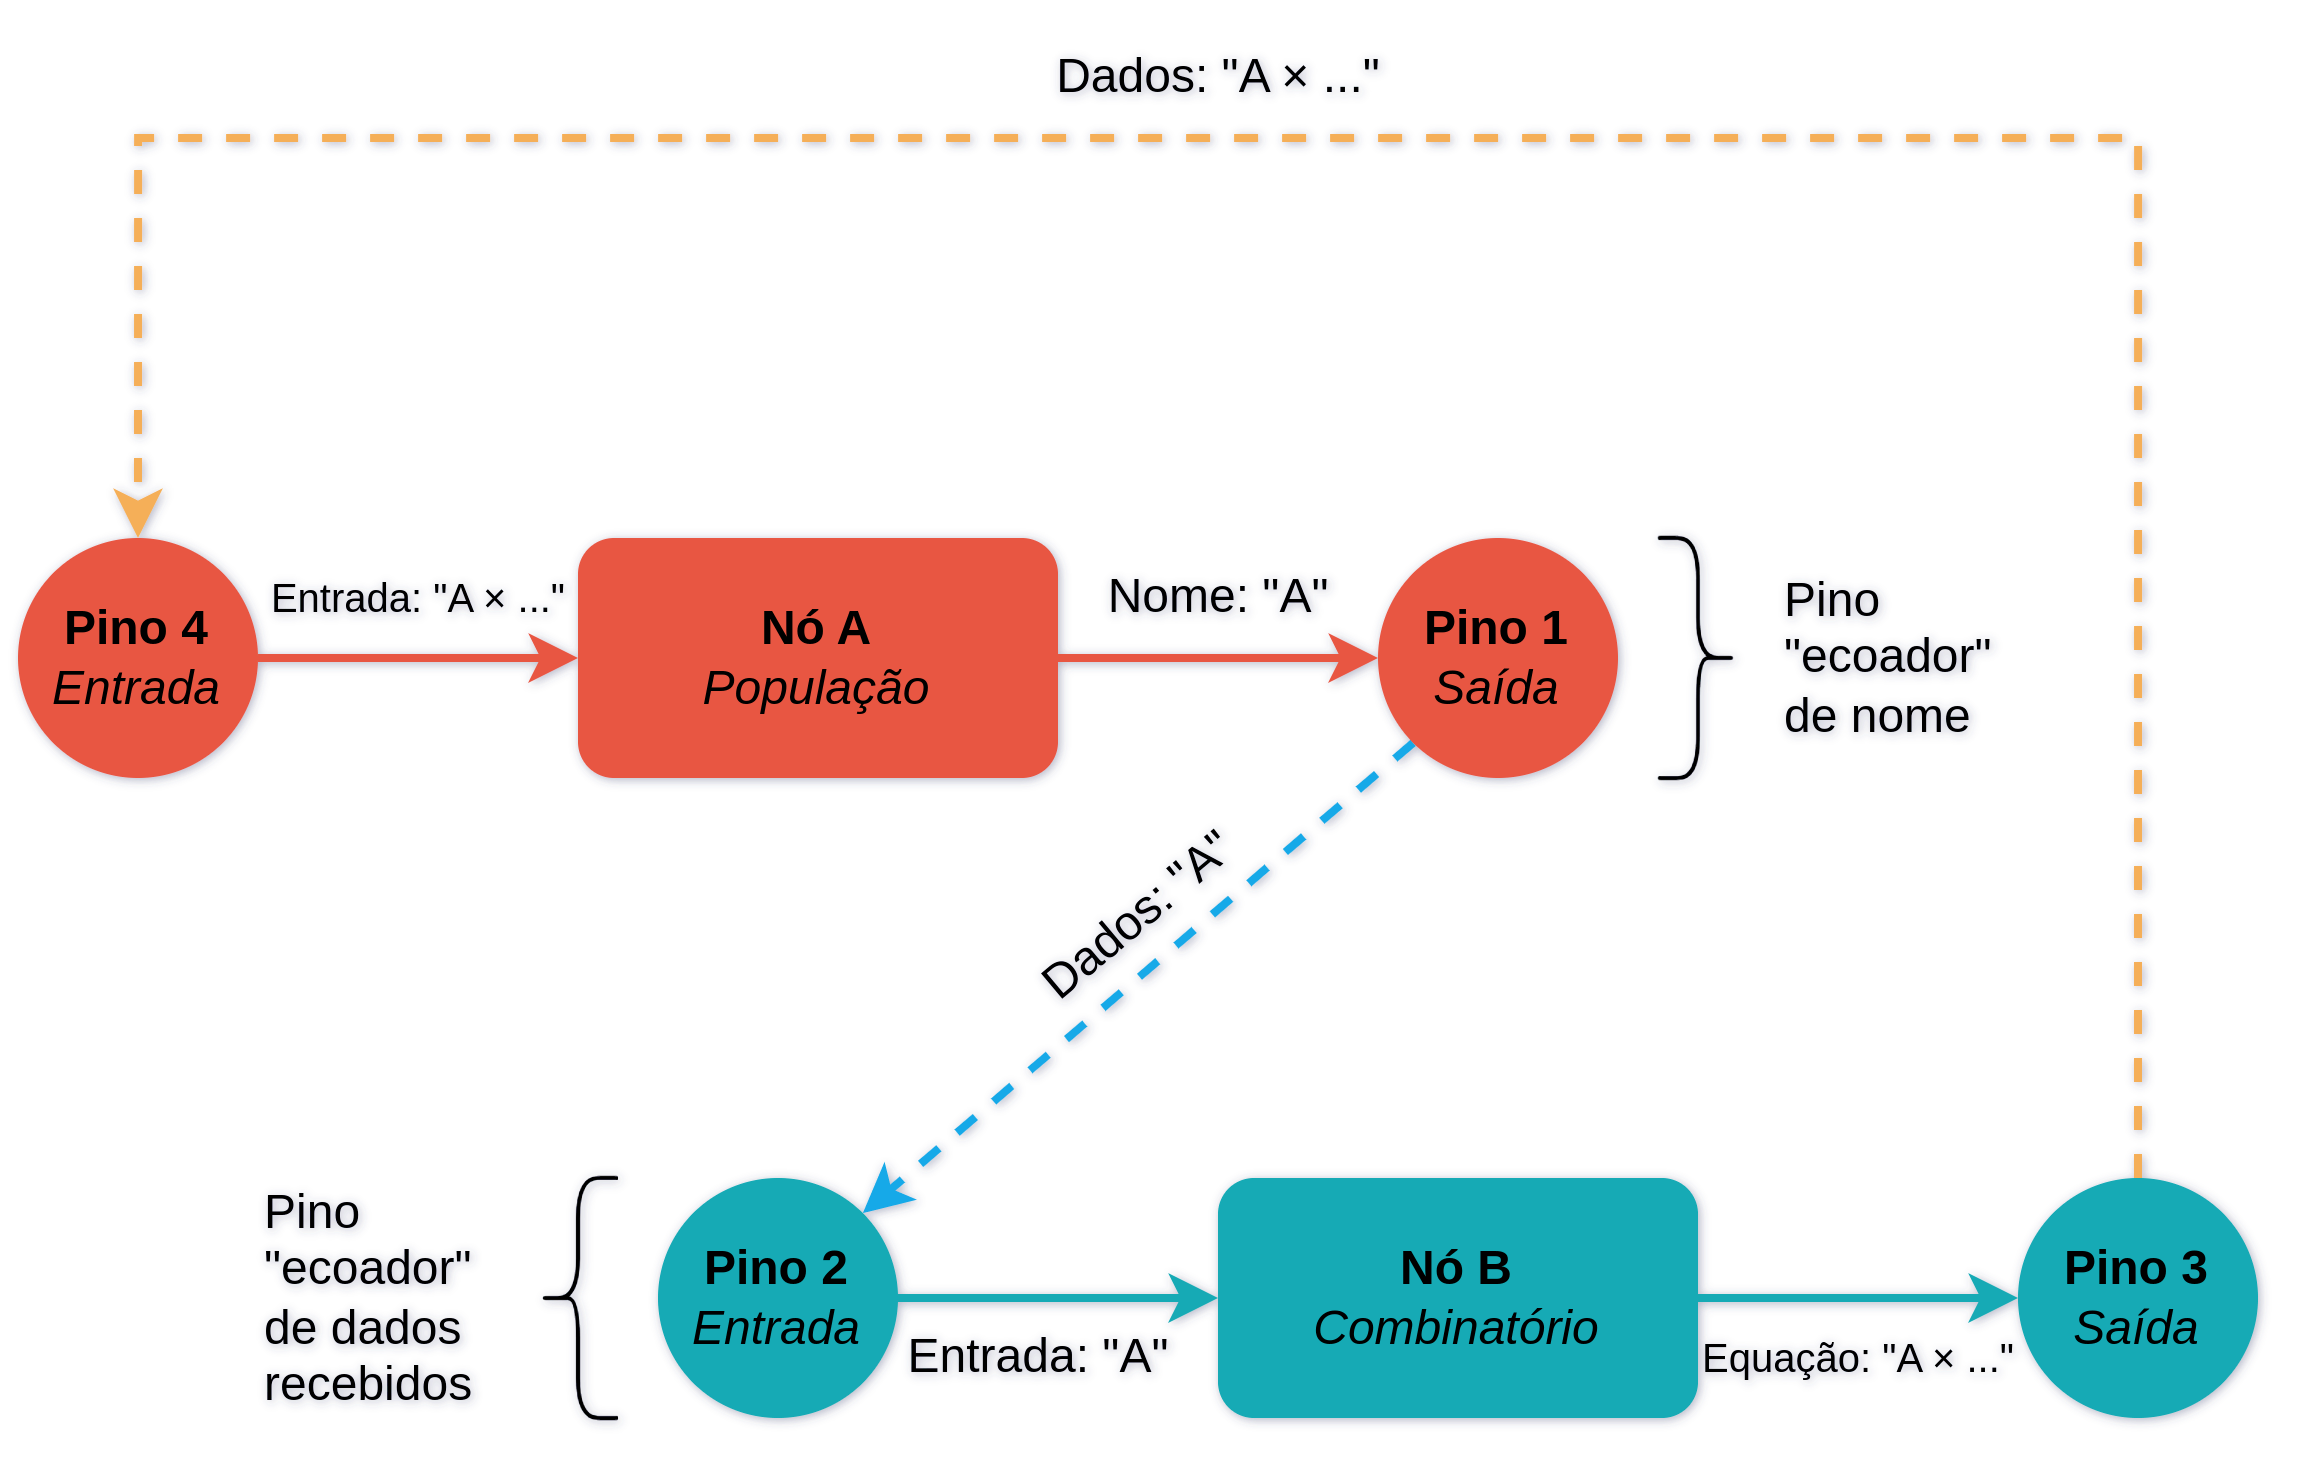
\includegraphics[scale=0.175]{imgs/fluxo_dados_gui.png} 
    \caption{Fluxo da passagem de dados entre nós e pinos na interface gráfica.}
    \label{fig::fluxo_dados_gui}
\end{figure}

A Figura \ref{fig::fluxo_dados_gui} ilustra como o nome da população ``A'' é levada até um nó combinatório que monta a expressão ``A * ...'' (assumindo nós omitidos) e retorna-o para a população, por meio de conexões entre pinos. É importante que as populações recebam as expressões montadas pelos combinadores para que o usuário consiga facilmente observar as equações completas a qualquer momento.

\subsection{A biblioteca de RI}
\label{subsec:biblioteca_RI}

Para realizar todas as conversões mencionadas ao longo deste texto, foi desenvolvida uma biblioteca em Rust. A linguagem Rust foi escolhida por trazer maior segurança, confiabilidade e facilidade de desenvolvimento. Como Rust é uma linguagem compilada, é possível compilar bibliotecas estáticas ou dinâmicas para utilizar em C ou C++. No caso deste software, a biblioteca expõe algumas \texttt{structs} e funções utilizando a \textit{FFI} (acrônimo para Interface de Funções Estrangeiras, em inglês) de C, e os arquivos \textit{headers} são gerados automaticamente pelo programa \textbf{cbindgen}\footnote{\href{https://github.com/eqrion/cbindgen}{https://github.com/eqrion/cbindgen}} e \textbf{GitHub Actions}\footnote{\href{https://github.com/marketplace/actions/cbindgen-action}{cbindgen-action}}.

O software utiliza a biblioteca \textbf{serde}\footnote{\href{https://serde.rs/}{https://serde.rs/}} para declarativamente criar as conversões das \texttt{structs} de/para o formato JSON por meio do macro \textit{derive} de Rust. Este macro permite que estruturas implementem certos métodos automaticamente, puramente pela leitura dos campos que esta possui. Este é o caso das \texttt{structs} \texttt{Model}, \texttt{MetaData}, \texttt{Node} e \texttt{Constant}.

Uma outra vantagem da linguagem Rust é possuir um ecossistema de bibliotecas com pequenos escopos e bem integradas. Neste caso, o motor de \textit{templates} utilizado, \textbf{minijinja}\footnote{\href{https://github.com/mitsuhiko/minijinja}{https://github.com/mitsuhiko/minijinja}}, recebe como entrada para suas conversões estruturas que implementam métodos de serialização e desserialização da biblioteca serde.

Pelos motivos mencionados acima, a implementação das conversões de/para JSON e para o modelo de EDOs foi tão simples quanto declarar as estruturas e escrever o \textit{template} de EDOs, apresentado em \ref{code::equation-template-jinja}.

\subsection{Testes unitários}

O software atualmente também implementa testes unitários em C++ utilizando o \textit{framework} de testes \textbf{Catch2}\footnote{\href{https://github.com/catchorg/catch2}{https://github.com/catchorg/catch2}}. O objetivo dos testes é garantir que a biblioteca em Rust é compilável e possui estruturas que passam de forma segura pela FFI de C. Adicionalmente, os testes realizam garantias como checagem de campos em JSON antes e pós conversão para estruturas.

Estes testes tornam a vida do desenvolvedor mais fácil, uma vez que garantem que alterações no código não quebram funcionalidades pré-existentes. Os testes possuem execução automatizada por meio de \textbf{GitHub Actions}\footnote{\href{https://github.com/features/actions}{GitHub Actions}}, que fornecem máquinas em nuvem sob demanda, assim impedindo que o desenvolvedor se descuide e esqueça de executá-los.

\subsection{Distribuição do software}

%TO DO: 
%Apesar do software utilizar diversas bibliotecas externas, foi criado uma App Image (Fuse 3, ref) 
%Falar do container 
%As dependências para a execução da App Image são somente um conjunto de bibliotecas padrão disponível em todos os sistemas baseados em Linux. 

\chapter{Resultados}
\label{chap:resultados}
%Mostrar exemplos de modelos construídos e simulados com a ferramenta 

%-----------------------------//----------------------------
\chapter{Conclusão e trabalhos futuros}
\label{chap:conclusao}
%e modelos estocásticos com o algoritmo de Gillespie

Desde o início do Mestrado até o presente momento, foram realizadas as seguintes atividades: 
\begin{itemize}
    \item Iterações de design para layout da interface gráfica;
    \item Prototipagem da interface gráfica;
    \item Implementação das principais funcionalidades e classes da interface gráfica utilizando a biblioteca ImGui;
    \item Implementação da Representação Intermediária e salvamento/carregamento de arquivos do computador;
\end{itemize}

Espera-se que, até o final deste ano, o software seja capaz de realizar o fluxo completo de salvamento/carregamento, criação do modelo, simulação \textit{onsite}, geração de código e exportação dos resultados das simulações em PDF.

Um trabalho futuro é desenvolver uma versão Web do software para que ele possa ser utilizado por um número maior de pessoas. A criação do modelo será feita através do navegador Web e todo o processamento incluindo a geração de código, execução, geração dos resultados e imagens será feita no servidor. As tecnologias usadas pelo projeto até então são todas compatíveis com a Web; para as linguagens C e C++ existe o projeto \textbf{Emscripten}\footnote{\href{https://emscripten.org/}{https://emscripten.org/}}, um compilador baseado na LLVM que é capaz de gerar WebAssembly. Já o Rust, também baseado na LLVM, possui suporte nativo à WebAssembly.

Outro trabalho futuro é a implementação da geração de código para modelos de Equações Diferenciais Parciais (EDPs) utilizando o método de diferenças finitas. Essa implementação iria exigir uma mudança maior na interface e na representação intermediária para acomodar características e recursos que são próprios de modelos de EDPs. 

Por último, destaca-se que uma outra possibilidade de extensão do trabalho é a implementação de funcionalidades para realizar a estimativa de parâmetros do modelo de EDOs e a análise de sensibilidade do modelo. Essas novas funcionalidades seriam integradas ao software existente.  

%TO DO: Falar das limitações do trabalho 
%Limitação da representação visual: Modelos mais complexos, muitos nós e ligações (fica difícil entender o modelo). 

%Solução: Uma ideia é oferecer a possibilidade de agrupar um grupo de nós e as ligações entre eles em um submodelo. Os submodelos seriam combinados para formar o modelo completo. 

% % ---
% % Finaliza a parte no bookmark do PDF, para que se inicie o bookmark na raiz
% % ---
% \bookmarksetup{startatroot}% 
% % ---

% % ---------------------------------------------------------------------------------------------
% % ---------------------------------------------------------------------------------------------
% % ----------------------------------------------------------------------ELEMENTOS PÓS-TEXTUAIS-
% % ---------------------------------------------------------------------------------------------
% % ---------------------------------------------------------------------------------------------
\postextual

% % ----------------------------------------------------------
% % Referências bibliográficas
% % ----------------------------------------------------------
\bibliographystyle{abntex2-alf}
\bibliography{referencias}

% % ---------------------------------------------------------------------------------------------
% % ------------------------------------------------------Apêndices - Caso não existam, comentar-
% % ---------------------------------------------------------------------------------------------
%\begin{apendicesenv}
	
	% Imprime uma página indicando o início dos apêndices
	\partapendices


\end{apendicesenv}

\appendix {

\section{Código de Python gerado para o modelo Predador-Presa}
\label{code:predador-presa}
\textattachfile{code/dhdp.py}{código completo}
\lstinputlisting[language=Python]{code/dhdp-part.py}

}

% % ---------------------------------------------------------------------------------------------
% % ---------------------------------------------------------Anexos - Caso não existam, comentar-
% % ---------------------------------------------------------------------------------------------
% %% ---
% Inicia os anexos
% ---
\begin{anexosenv}

% Imprime uma página indicando o início dos anexos
\partanexos

% ---
\chapter{Morbi ultrices rutrum lorem.}
% ---

Lorem ipsum dolor sit amet, consectetur adipiscing elit. Maecenas laoreet porttitor dui sit amet tempus. Phasellus finibus ac tortor eget lobortis. Suspendisse et nunc velit. Vestibulum vulputate, urna laoreet hendrerit dignissim, urna massa facilisis ante, quis vestibulum erat elit blandit eros. Cras a justo eu risus lobortis lobortis vitae luctus mauris. Nunc congue consequat justo, eget imperdiet magna porttitor nec. Class aptent taciti sociosqu ad litora torquent per conubia nostra, per inceptos himenaeos. Vestibulum lorem ex, vulputate nec nibh ac, consequat vulputate ex. Aliquam dignissim dapibus orci, eget porttitor dui rutrum a. Pellentesque lacinia ante in sapien lacinia, a ultrices libero faucibus. In erat purus, elementum ut lectus nec, iaculis accumsan mi. Donec bibendum ante ac nulla hendrerit consectetur. Aliquam a mauris ultricies, ornare lacus sed, convallis orci. Class aptent taciti sociosqu ad litora torquent per conubia nostra, per inceptos himenaeos.

Etiam viverra risus non sodales vehicula. In convallis sapien vel neque aliquam, non porttitor turpis dapibus. Suspendisse consectetur volutpat purus, quis ultrices odio tempor id. Duis laoreet justo quam, vitae ultrices tellus dapibus vel. Mauris placerat ipsum finibus odio luctus suscipit. Duis facilisis non leo non varius. Sed et magna feugiat, rutrum diam vel, maximus nunc.

% ---
\chapter{Cras non urna sed feugiat cum sociis natoque penatibus et magnis dis
parturient montes nascetur ridiculus mus}
% ---


Lorem ipsum dolor sit amet, consectetur adipiscing elit. Maecenas laoreet porttitor dui sit amet tempus. Phasellus finibus ac tortor eget lobortis. Suspendisse et nunc velit. Vestibulum vulputate, urna laoreet hendrerit dignissim, urna massa facilisis ante, quis vestibulum erat elit blandit eros. Cras a justo eu risus lobortis lobortis vitae luctus mauris. Nunc congue consequat justo, eget imperdiet magna porttitor nec. Class aptent taciti sociosqu ad litora torquent per conubia nostra, per inceptos himenaeos. Vestibulum lorem ex, vulputate nec nibh ac, consequat vulputate ex. Aliquam dignissim dapibus orci, eget porttitor dui rutrum a. Pellentesque lacinia ante in sapien lacinia, a ultrices libero faucibus. In erat purus, elementum ut lectus nec, iaculis accumsan mi. Donec bibendum ante ac nulla hendrerit consectetur. Aliquam a mauris ultricies, ornare lacus sed, convallis orci. Class aptent taciti sociosqu ad litora torquent per conubia nostra, per inceptos himenaeos.

Etiam viverra risus non sodales vehicula. In convallis sapien vel neque aliquam, non porttitor turpis dapibus. Suspendisse consectetur volutpat purus, quis ultrices odio tempor id. Duis laoreet justo quam, vitae ultrices tellus dapibus vel. Mauris placerat ipsum finibus odio luctus suscipit. Duis facilisis non leo non varius. Sed et magna feugiat, rutrum diam vel, maximus nunc.

Donec vehicula dapibus pharetra. Etiam et libero pharetra nulla ultricies laoreet sit amet vel sapien. Proin ultrices vitae nibh quis accumsan. Nullam in tortor erat. Quisque imperdiet dui venenatis pulvinar laoreet. Nulla ut nunc sed urna consectetur finibus id ut justo. Sed in placerat massa, quis tempor orci.


\end{anexosenv}

% %---------------------------------------------------------------------
% % INDICE REMISSIVO
% %---------------------------------------------------------------------
% %\printindex

\end{document}
